\newcommand{\titleinfo}{Wavelets}
\newcommand{\subjectinfo}{From Fourier To Wavelets}
\newcommand{\authorinfo}{Gian Danuser}
\newcommand{\versioninfo}{0.1}
\newcommand{\newpar}{\par\par}

%%%%%%%%%%%%%%%%%%%%%%%%%%%%%%%%%%%%%%%%%%
% Dokument
%%%%%%%%%%%%%%%%%%%%%%%%%%%%%%%%%%%%%%%%%%
\documentclass[11pt,twoside]{scrartcl} %oneside Change xxxside -->marginpar must bee changed

\usepackage[pdftitle={\titleinfo},%
						pdfauthor={\authorinfo},%
						pdfcreator={pdfLatex, LaTeX with hyperref},
						pdfsubject={\subjectinfo},
						plainpages=false,
						pdfpagelabels,
						colorlinks,
						linkcolor=black,
						filecolor=black,
						citecolor=black,
						urlcolor=black]{hyperref}
						

% Headings
\usepackage{fancyhdr}
\renewcommand{\headrulewidth}{0.4pt}
\renewcommand{\footrulewidth}{0.4pt}	

\lhead[\scriptsize\nouppercase{\leftmark}]{\textbf{\titleinfo}}
\chead[V\versioninfo]{V\versioninfo}
\rhead[\textbf{\titleinfo}]{\scriptsize\nouppercase{\leftmark}}

\lfoot[\thepage]{\authorinfo}
\cfoot[]{}
\rfoot[\authorinfo]{\thepage}


%%%%%%%%%%%%%%%%%%%%%%%%%%%%%%%%%%%%%%%%%%
% Package's
%%%%%%%%%%%%%%%%%%%%%%%%%%%%%%%%%%%%%%%%%%
\usepackage{ucs}
\usepackage[utf8x]{inputenc}
\usepackage[T1]{fontenc}

\usepackage{layout}
\setlength{\parindent}{0em}

\usepackage{lscape}

\renewcommand{\baselinestretch}{1.2}
\renewcommand{\arraystretch}{1}

%Damit \today ein Deutsch Formatiertes Datum zurueckgibt.
\usepackage[ngerman, num, orig]{isodate}
\usepackage[german, ngerman]{babel}
\monthyearsepgerman{\,}{\,}

\usepackage{amssymb,amsmath,fancybox,graphicx,wrapfig,color,lastpage,verbatim,epstopdf,a4wide,tabularx, pdftricks}
\usepackage[usenames,dvipsnames]{pstricks}
\usepackage{setspace}
\usepackage{epsfig}
\usepackage{pst-pdf}
\usepackage{pst-all}
\usepackage{pstricks-add}
\usepackage{supertabular}
\usepackage[font=small,labelfont=bf]{caption}
\usepackage[font=footnotesize]{subfig}
\usepackage{footnote}
\usepackage{float}
\usepackage{multirow}
\usepackage{etex}
\usepackage{pdfpages}
\usepackage{pgf,tikz}
\usepackage{color}

\usepackage[makeroom]{cancel}
\usepackage{array}
\usepackage{trfsigns}
\usepackage{textcomp}


\renewcommand{\captionfont}{\scriptsize\slshape}

%Neue Symbole für itemize
\newcommand{\cditem}[2]{\item[$\blacktriangleright$] \textbf{#1} \\ #2}
\newcommand{\cdrawitem}[1]{\item[$\blacktriangleright$] \textbf{#1}}
\newcommand{\cdsubitem}[2]{\item[$\vartriangleright$] \textbf{#1} \\ #2}

\newcommand{\fullquote}[2]{
	\begin{verse}
	 	\centering\emph{#1}
	\end{verse}
	
	\begin{flushright}
		$-$ \emph{#2}
	\end{flushright}
}
	
\setlength{\unitlength}{1mm}

%Inhaltsverzeichnis
\setcounter{secnumdepth}{3}
\setcounter{tocdepth}{3}

%Geometrie
\usepackage[a4paper,left=10mm,right=10mm,top=10mm,bottom=10mm,includeheadfoot]{geometry}

%%%%%%%%%%%%%%%%%%%%%%%%%%%%%%%%%%%%%%%%%%
% Randnotizen 
%%%%%%%%%%%%%%%%%%%%%%%%%%%%%%%%%%%%%%%%%%

%\setlength{\marginparwidth}{20mm} %Legt die Breite des Randnotizen-Bereichs fest.
%\setlength{\marginparpush}{10mm} %Legt den minimalen Abstand zwischen zwei Randnotizen fest.
%\setlength{\marginparsep}{3mm} %Legt den Abstand zwischen Text und Randnotizen fest.

%Info: Twosided
%\let\oldmarginpar\marginpar
%\renewcommand{\marginpar}[1]{
%	\ifthenelse{\isodd{\thepage}}
%	{ %then clause (gerade seiten)
%		\reversemarginpar
%		\vspace{\baselineskip}
%		\oldmarginpar[\raggedleft\footnotesize\textbf{#1}]{\raggedleft\footnotesize\textbf{#1}}
%		\normalmarginpar
%		\vspace{\baselineskip}
%		\oldmarginpar[\raggedleft\footnotesize\textbf{#1}]{\raggedleft\footnotesize\textbf{#1}}
%		\vspace{-\baselineskip}
%	}
%}

%Info: Onesided
%\let\oldmarginpar\marginpar
%\renewcommand{\marginpar}[1]{
%	\reversemarginpar
%	\vspace{\baselineskip}
%	\oldmarginpar[\raggedleft\footnotesize\textbf{#1}]{\raggedleft\footnotesize\textbf{#1}}
%	\vspace{-\baselineskip}
%}



%%%%%%%%%%%%%%%%%%%%%%%%%%%%%%%%%%%%%%%%%%
% Code Listings
%%%%%%%%%%%%%%%%%%%%%%%%%%%%%%%%%%%%%%%%%%
\usepackage{listings}
\definecolor{listinggray}{gray}{0.9}
\definecolor{lbcolor}{rgb}{0.95,0.95,0.95}
\definecolor{comment}{RGB}{34, 139, 34}
\lstset{
	backgroundcolor=\color{lbcolor},
	tabsize=4,
	rulecolor=,
	numbers=left,
	basicstyle=\scriptsize,
	upquote=true,
	aboveskip={1.0\baselineskip},
	columns=fixed,
	showstringspaces=false,
	extendedchars=true,
	breaklines=true,
	prebreak = \raisebox{0ex}[0ex][0ex]{\ensuremath{\hookleftarrow}},
	frame=single,
	showtabs=false,
	showspaces=false,
	showstringspaces=false,
	identifierstyle=\ttfamily,
	keywordstyle=\color[rgb]{0,0,1},
	commentstyle=\color{comment},
	stringstyle=\color{brown}, %\color[rgb]{0.627,0.126,0.941},
	captionpos=b,
}

\lstset{
	language=C++,
	directivestyle=\color{brown},	
}

\lstdefinelanguage[STL]{C++} [ANSI]{C++}{
	morekeywords=[2]{string, vector, list, map, std},
	%morecomment=[s]{{<}{>}},
	%commentstyle=\color{comment}
}

\lstdefinelanguage[Qt]{C++} [ANSI]{C++}{
	morekeywords=[2]{slot, signal, emit, foreach},
	morekeywords=[3]{slot, signal, emit, foreach}.
}

\lstdefinelanguage{cmd}{
	morecomment=[l]{\#},
	commentstyle=\color{comment}
}



%%%%%%%%%%%%%%%%%%%%%%%%%%%%%%%%%%%%%%%%%%%%%%%%%%%%%%%%%%%%%%%%
% Referenzen
%%%%%%%%%%%%%%%%%%%%%%%%%%%%%%%%%%%%%%%%%%%%%%%%%%%%%%%%%%%%%%%%

\newcommand{\figref}[1]{Abb.~\ref{#1}}
\newcommand{\subfigref}[2]{\figref{#1}.#2}
\renewcommand{\eqref}[1]{Gl.~\ref{#1}}
\newcommand{\tabref}[1]{Tabelle~\ref{#1}}
\renewcommand{\pageref}[1]{Seite~\ref{#1}}
\newcommand{\chapref}[1]{Kapitel~\ref{#1}}
\newcommand{\secref}[1]{Abschnitt~\ref{#1}}
\newcommand{\lstref}[1]{Listing~\ref{#1}}



%%%%%%%%%%%%%%%%%%%%%%%%%%%%%%%%%%%%%%%%%%%%%%%%%%%%%%%%%%%%%%%%
% Environment Numbering
%%%%%%%%%%%%%%%%%%%%%%%%%%%%%%%%%%%%%%%%%%%%%%%%%%%%%%%%%%%%%%%%

%Abbildungsnumerierung anhand Kapitel
\renewcommand{\thefigure}{\arabic{section}.\arabic{figure}}
\makeatletter \@addtoreset{figure}{section} \makeatother

%Gleichungen anhand Kapitel
\AtBeginDocument{\numberwithin{equation}{section}}
\AtBeginDocument{\numberwithin{figure}{section}}
\AtBeginDocument{\numberwithin{lstlisting}{section}}
\AtBeginDocument{\numberwithin{table}{section}}



%%%%%%%%%%%%%%%%%%%%%%%%%%%%%%%%%%%%%%%%%%%%%%%%%%%%%%%%%%%%%%%%
% Mathe
%%%%%%%%%%%%%%%%%%%%%%%%%%%%%%%%%%%%%%%%%%%%%%%%%%%%%%%%%%%%%%%%
\DeclareMathOperator{\sinc}{sinc}

\newcommand{\numbercircled}[1]{\textcircled{\raisebox{-1pt}{#1}}}

% Fouriertransformationen
\unitlength1cm
\newcommand{\FT}
{
	\begin{picture}(1,0.5)
	\put(0.2,0.1){\circle{0.14}}\put(0.27,0.1){\line(1,0){0.5}}\put(0.77,0.1){\circle*{0.14}}
	\end{picture}
}

% Inverse- Fouriertransformation
\newcommand{\IFT}
{
	\begin{picture}(1,0.5)
	\put(0.2,0.1){\circle*{0.14}}\put(0.27,0.1){\line(1,0){0.45}}\put(0.77,0.1){\circle{0.14}}
	\end{picture}
}



%%%%%%%%%%%%%%%%%%%%%%%%%%%%%%%%%%%%%%%%%%%%%%%%%%%%%%%%%%%%%%%%
% Farben
%%%%%%%%%%%%%%%%%%%%%%%%%%%%%%%%%%%%%%%%%%%%%%%%%%%%%%%%%%%%%%%%

%Farben
\definecolor{black}{rgb}{0,0,0}
\definecolor{red}{rgb}{1,0,0}
\definecolor{white}{rgb}{1,1,1}
\definecolor{grey}{rgb}{0.8,0.8,0.8}

%Markierungen
\newcommand{\draftmarker}[1]{\colorbox{yellow}{#1}}



%%%%%%%%%%%%%%%%%%%%%%%%%%%%%%%%%%%%%%%%%%%%%%%%%%%%%%%%%%%%%%%%
% Tabellen
%%%%%%%%%%%%%%%%%%%%%%%%%%%%%%%%%%%%%%%%%%%%%%%%%%%%%%%%%%%%%%%%

%\renewcommand{\arraystretch}{1.5} %Zeilenh�he von Tabellen

\newcolumntype{L}[1]{>{\raggedright\arraybackslash}p{#1}} % linksbündig mit Breitenangabe
\newcolumntype{C}[1]{>{\centering\arraybackslash}p{#1}} % zentriert mit Breitenangabe
\newcolumntype{R}[1]{>{\raggedleft\arraybackslash}p{#1}} % rechtsbündig mit Breitenangabe

\newcommand{\ltab}{\raggedright\arraybackslash} % Tabellenabschnitt linksb�ndig
\newcommand{\ctab}{\centering\arraybackslash} % Tabellenabschnitt zentriert
\newcommand{\rtab}{\raggedleft\arraybackslash} % Tabellenabschnitt rechtsb�ndig




%%%%%%%%%%%%%%%%%%%%%%%%%%%%%%%%%%%%%%%%%%%%%%%%%%%%%%%%%%%%%%%%
% Einheiten
%%%%%%%%%%%%%%%%%%%%%%%%%%%%%%%%%%%%%%%%%%%%%%%%%%%%%%%%%%%%%%%%
\usepackage[Gray,squaren]{SIunits} %\gray befehl heisst nun \Gray und \square heisst nun \squaren

%Spannung
\DeclareMathOperator{\V}{\volt}
\DeclareMathOperator{\mV}{\milli \volt}
\DeclareMathOperator{\uV}{\micro \volt}

%Strom
\DeclareMathOperator{\A}{\ampere}
\DeclareMathOperator{\mA}{\milli \ampere}
\DeclareMathOperator{\uA}{\micro \ampere}
\DeclareMathOperator{\nA}{\nano \ampere}

%Zeit
\DeclareMathOperator{\s}{\second}
\DeclareMathOperator{\ms}{\milli \second}
\DeclareMathOperator{\us}{\micro \second}
\DeclareMathOperator{\ns}{\nano \second}

%Kapazit�t
\DeclareMathOperator{\mF}{\milli \farad}
\DeclareMathOperator{\uF}{\micro \farad}
\DeclareMathOperator{\nF}{\nano \farad}
\DeclareMathOperator{\pF}{\pico \farad}
\DeclareMathOperator{\fF}{\femto \farad}

%Induktivit�t
\DeclareMathOperator{\mH}{\milli \henry}
\DeclareMathOperator{\uH}{\micro \henry}
\DeclareMathOperator{\nH}{\nano \henry}

%Widerstand
\DeclareMathOperator{\MO}{\mega \ohm}
\DeclareMathOperator{\kO}{\kilo \ohm}
\DeclareMathOperator{\mO}{\milli \ohm}
\DeclareMathOperator{\Ohm}{\ohm}
%Strecke
\DeclareMathOperator{\km}{\kilo \meter}
\DeclareMathOperator{\cm}{\centi \meter}
\DeclareMathOperator{\mm}{\milli \meter}

%Frequenz
\DeclareMathOperator{\GHz}{\giga \hertz}
\DeclareMathOperator{\MHz}{\mega \hertz}
\DeclareMathOperator{\Hz}{\hertz}
\DeclareMathOperator{\kHz}{\kilo \hertz}
\DeclareMathOperator{\mHz}{\milli \hertz}

%Leistung
\DeclareMathOperator{\kW}{\kilo \watt}
\DeclareMathOperator{\mW}{\milli \watt}
\DeclareMathOperator{\uW}{\micro \watt}
\DeclareMathOperator{\W}{\watt}

%Kreisfrequenz
\DeclareMathOperator{\rpers}{\radianpersecond}

%DeziBel
\DeclareMathOperator{\dB}{\deci \bel}
\DeclareMathOperator{\dBm}{\deci \bel \milli}

%Bit
\DeclareMathOperator{\Bit}{\text{Bit}}
\DeclareMathOperator{\kBit}{\text{kBit}}
\DeclareMathOperator{\MBit}{\text{MBit}}
\DeclareMathOperator{\Byte}{\text{Byte}}
\DeclareMathOperator{\kByte}{\text{kByte}}
\DeclareMathOperator{\MByte}{\text{MByte}}
\DeclareMathOperator{\ppm}{\text{ppm}}



\newcommand{\todo}[1]{\colorbox{red}{#1}}

\begin{document}
		
% % % % % % % % % % % % % % % % % % % % % % % % % % % % % % % %
% Kapitel
% % % % % % % % % % % % % % % % % % % % % % % % % % % % % % % %
	%Kopf und Fuszeile aktivieren
	\pagestyle{fancy}
	
	%damit " kein umlaut erzeugt und als Anführungszeichn verwendet werden kann
	\shorthandoff{"} %Abschalten mit \shorthandon{"}
	
	%Titel
	{\LARGE\textbf{\subjectinfo}}
	
	Bemerkung zum Dokument:\\
	$e$ orthonormale Basisvektoren, $b$ Basisvektor, $d$ duale Basis zu $b$\\
	Vektoren: Kleinbuchstaben fett, Matrize: Grossbuchstaben fett, Konstanten: Kleinbuchstaben\\
	$(\cdots)^*$ konjugiert Komplex,
		
	%Includes	
	\section{Grundlagen}

\subsection{Skalarprodukt}

Vektor:
\[
	\langle \mathbf{v}|\mathbf{w}\rangle = v_1^* \cdot w_1 + v_2^* \cdot w_2 + ... + v_n^* \cdot w_n  \in \mathbb{R} \qquad \qquad \mathbf{v},\mathbf{ w} \in \mathbb{R} \text{ oder } \in \mathbb{C} 
\]

Funktion:
\[  
	\langle f(t)|g(t) \rangle =  \int f(t)^*\cdot g(t) \,\mathrm{d}t \in \mathbb{R} \qquad \qquad g(t), f(t) \in \mathbb{R} \text{ oder } \in \mathbb{C}
\]
Grenzen werden situationsabhängig festgelegt, z.B.: Polynome [-1,1], T periodische Funktionen [0,T] oder [-T/2,T/2], Funktionen in $\mathbb{R}$ von $[-\infty,\infty]$ etc. (Funktion entspricht Vektor mit $\infty$ Elementen)

\subsubsection{Eigenschaften}
Symmetrie: $\langle v_1|v_2 \rangle = \langle v_2|v_1 \rangle^* \, \in \mathbb{C}  \qquad \langle v_1|v_2 \rangle = \langle v_2|v_1 \rangle \, \in \mathbb{R}$ \\
Linear: $\langle v_1|v_2 + v_3 \rangle = \langle v_1|v_2 \rangle + \langle v_1|v_3 \rangle =\langle v_1 + v_2|v_3 \rangle = \cdots  \qquad \text{und}\qquad \langle \lambda \cdot v_1|v_2 \rangle = \lambda \langle v_1|v_2 \rangle = \langle v_1|\lambda \cdot v_2 \rangle$\\
Positiv: $||v||^2 = \langle v|v \rangle \geq 1 \qquad \text{Ausnahme:} \, ||v||^2=0 \, \text{wenn} \, v=0$\\
Definition der Länge von $v$ (bei Funktionen Norm genannt): $||v|| = \sqrt{\langle v|v \rangle} = \sqrt{||v||^2}$\\
Definition des Winkels $\gamma$ zwischen $v$ und $w$: $cos(\gamma) = \frac{\langle v|w \rangle}{||v||\cdot ||w||} \qquad$ wenn $v \perp w  \quad \langle v|w \rangle = 0$


\subsection{Basis eines Vektorraums}
Jeder n-dimensionale Vektorraum $V$ wird von n Basisvektoren $B=\{ b_1,...,b_n \}$ aufgespannt. Jeder Vektor, der sich in diesem Vektorraum befindet, kann als Linearkombination der Basisvektoren dargestellt werden.  Alle Basisvektoren sind linear unabhängig voneinander (ein Basisvektor kann nicht durch Linearkombination der anderen Basisvektoren dargestellt werden)!

\[  
	v = \sum_{i=1}^{n}c_i \cdot b_i \qquad \qquad  b_k \neq \sum_{i=1 \, (i\neq k)}^{n}c_i \cdot b_i \qquad \qquad v \in V \quad c_i \in \mathbb{R}\text{ oder } \in \mathbb{C} \text{ bei complexem $V$}
\]

Jede Basis $b_i$ besitzt eine duale Basis $d_i$, wobei gilt: $\qquad \langle d_i|b_j\rangle = \delta_{ij} = \begin{cases} 1 \quad i=j\\ 0 \quad sonst  \end{cases}$

Wenn die Basisvektoren orthogonal sind, ist die duale Basis gleich der normalen Basis $b_i = d_i$.

Eine Basis ist orthonormal wenn die Basisvektoren $e_i$ orthogonal zueinander sind und jeweils die Länge 1 haben. Die duale Basis kann wie folgt berechnet werden. (Ohne Transponieren sind die Zeilenvektoren die dualen Basisvektoren!)

\[  
	B = \left[ b_1 \, b_2 \, \cdots \, b_n \right] \Rightarrow D=(B^{-1})^T = \left[ d_1 \, d_2 \, \cdots \, d_n \right]
\]

\[
	v=\sum_{i=1}^{n} \underbrace{\langle d_i|v \rangle}_{c_i} \cdot b_i = \sum_{i=1}^{n} \langle b_i|v \rangle \cdot d_i = B \cdot \underbrace{(D \cdot v)}_{c}
	\qquad \qquad 
	\left( \text{ orthonormiert: } v=\sum_{i=1}^{n} \underbrace{\langle e_i|v \rangle}_{c_i} \cdot e_i \right) 
\]


\subsection{Allgemeiner Satz des Pythagoras}

\[  
	||f-f_n||^2 =  ||f||^2 - \sum_{k=0}^{n} |c_k|^2 \qquad \qquad \left( n\rightarrow \infty: \quad ||f||^2=\sum_{k=0}^{n} |c_k|^2 \right)
\]


\subsection{Funktionsraum}
$L^2(\mathbb{R}) \qquad$ Menge der quadratintegrierbaren Funktionen $\int_{-\infty}^{\infty}|f(t)|^2 \mathrm{d}t < \infty$ oder $L^2(T) \quad \int_{0}^{T}|f(t)|^2 \mathrm{d}t < \infty$

($L^2(\mathbb{R})$ und $L^2(T)$ sind Hilberträume, da sie ein Skalarprodukt mit gewissen Axiomen erfüllt.)

$L^2$-Norm $||f-f_n|| \qquad$ Mass für die Güte der Approximation $f_n$ von der Funktion $f$

$L(\mathbb{R}) \qquad \int_{-\infty}^{\infty}|f(t)| \mathrm{d}t < \infty$ oder $L(T) \qquad \int_{0}^{T}|f(t)|^2 \mathrm{d}t < \infty$

\subsection{Punktweise Konvergenz}
$f(t) = f(t+T)$, $f(t) \in L^2([0,T])$ und $f'(t)$ existiert und ist kontinuierlich für alle $t \in \mathbb{R}$, dann konvergieren die Summen auch punktweise.

	\newpage
	\section{Wavelets}
\subsection{Allgemein \baeni{19}}
  Wavelet-Funktionen werden auch als \em Mother-Funktionen \em bezeichnet.
  \[
    \psi(t) = \psi_{0,0}(t)
  \]
 
  Davon werden gestreckte ($m>0$)/gestauchte ($m<0$) und verschobene (rechts: $n > 0$, links: $n < 0$) Funktionen hergeleitet:
  \[  
    \psi_{m,n}(t)=\frac{1}{\sqrt{2^m}} \cdot \psi\left(\frac{t}{2^m} - n\right) = 2^{-m/2} \cdot \psi(2^{-m}t-n) \quad m,n \in \mathbb{Z}
  \]
  Diese erfüllen die L2-Norm 1: $|| \psi_{m,n} ||^2 = \int_{-\infty}^{\infty} |\psi_{m,n}(t)|^2 dt = 1$ und sind orthonormiert: $<\psi_{m,n}, \psi_{m',n'}> = 0$, wenn $m \neq m'$ oder $n \neq n'$. Deren Mittelwert ist 0 (das 0. Moment ist verschwindend): $\int_{-\infty}^{\infty} \psi_{m,n}(t) dt = 0$.

\subsection{Haar Wavelets \baeni{19}}
\begin{center}
	\begin{minipage}[c]{0.65\textwidth}
    \begin{center}
    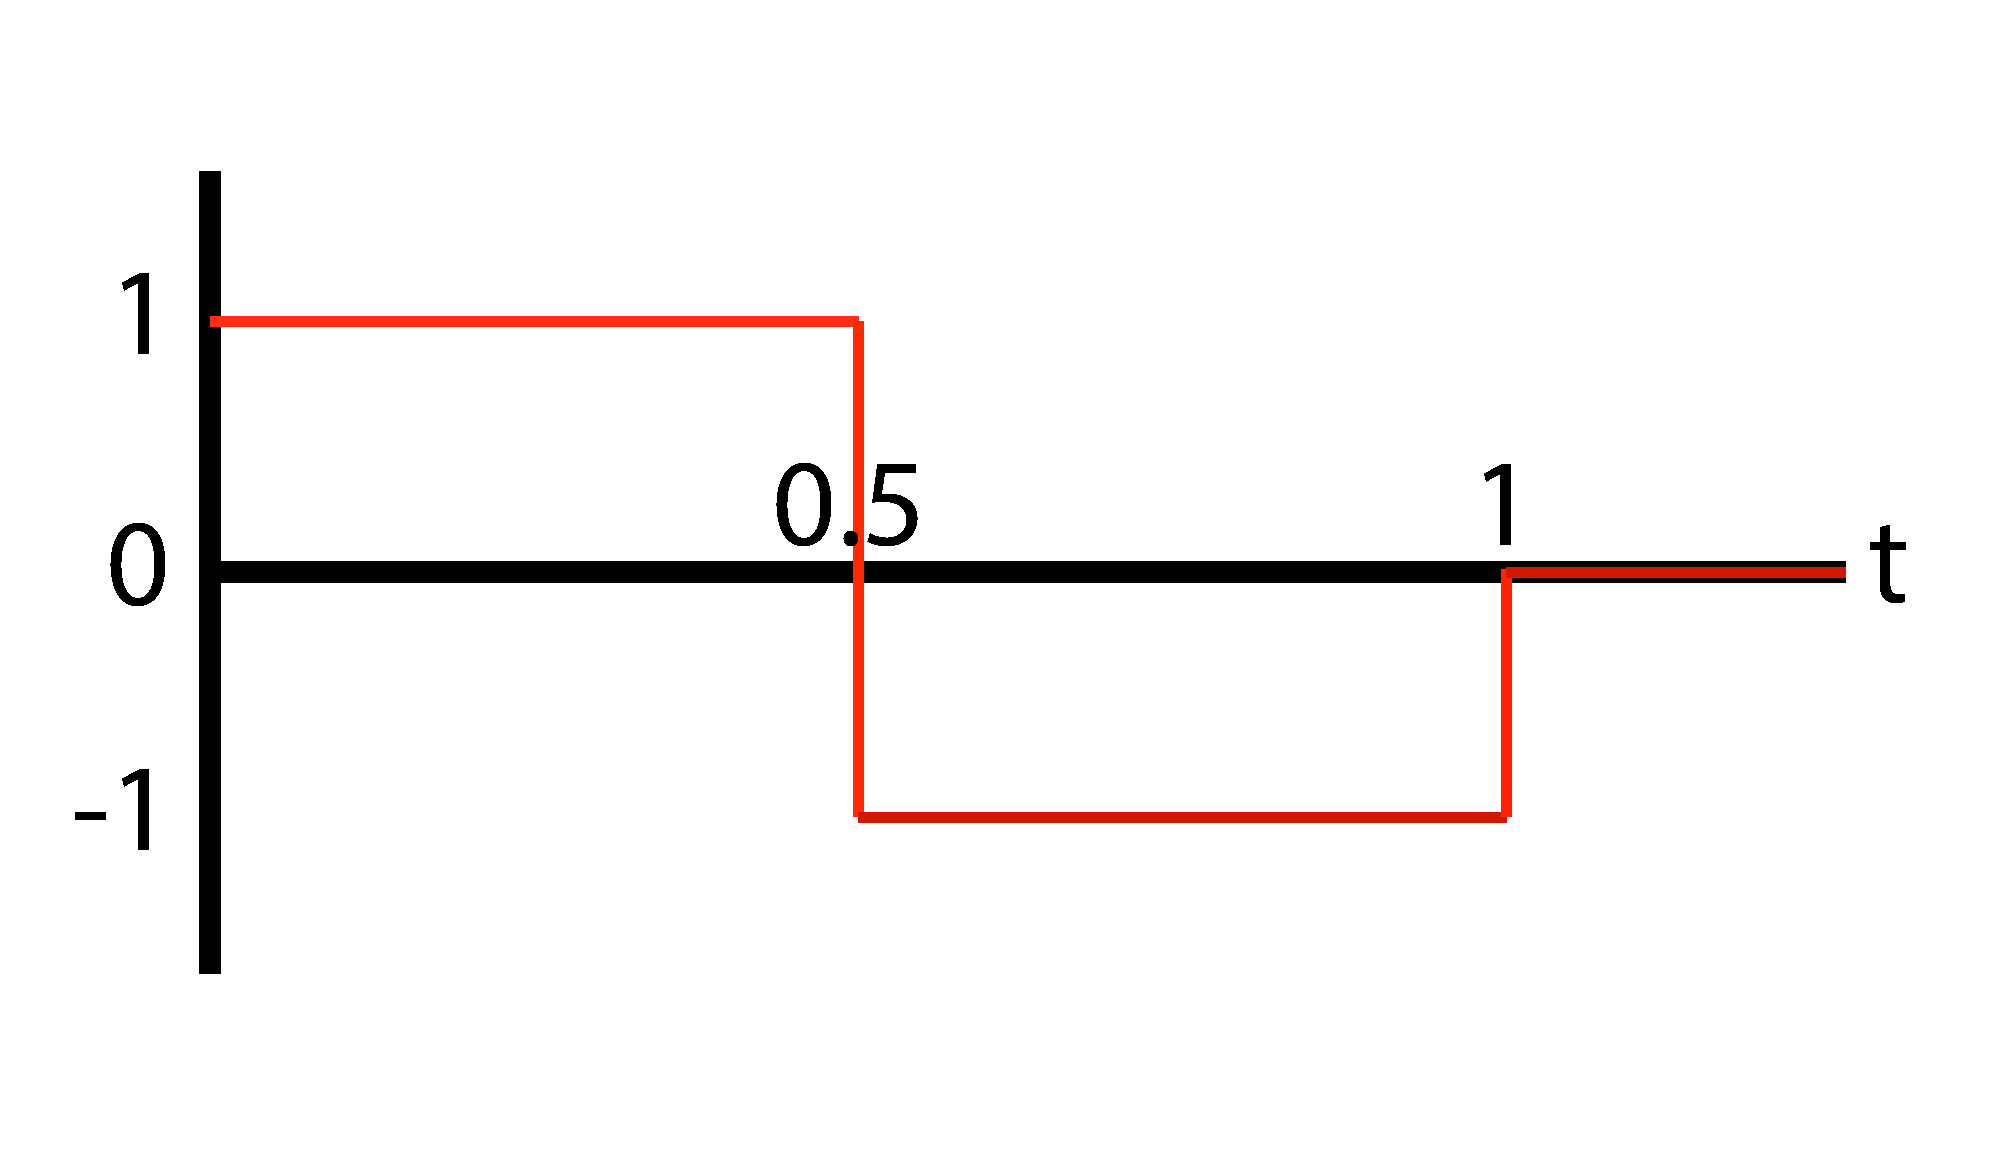
\includegraphics[width=6cm]{content/HaarWavelet.pdf}
    \end{center}
    \[
      \psi(t) = \psi_{0,0}(t)=\begin{cases} 1 \quad 0 \leq t < \frac{1}{2}\\ -1 \quad \frac{1}{2} \leq t < 1  \end{cases}
    \]
    
    \[	\psi_{m,n}  = \begin{cases} 
    	\frac{1}{\sqrt{2^m}} \qquad 2^m n \leq t < 2^m(n+\frac{1}{2}) \\ 
    	\frac{-1}{\sqrt{2^m}} \qquad 2^m(n+\frac{1}{2}) \leq t < 2^m(n+1)
    	\end{cases}
    \]
    
	\end{minipage}
	\begin{minipage}{0.3\textwidth}
	\textbf{Haar-Wavelets gestreckt, gestaucht und geschoben}\\
	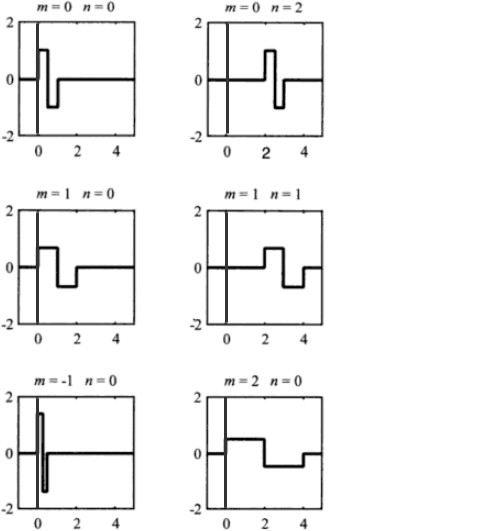
\includegraphics[width=7cm]{./Content/HaarStretchedMoved}
	\end{minipage}
\end{center}



\[ 
	\nu_{m,n} = \langle \psi_{m,n} | f \rangle = \int\limits_{-\infty}^{\infty}\psi_{m,n}(t) \cdot f(t) \,\mathrm{d}t = 
	\dfrac{1}{\sqrt{2^m}} \left( \int\limits_{2^mn}^{2^m(\frac12+n)} f(t) \mathrm{d}t - \int\limits_{2^m(\frac12+n)}^{2^m(1+n)}f(t) \mathrm{d}t  \right)
	\quad \Leftrightarrow \quad
	f(t)=\sum_{m,n \in \mathbb{Z}} \nu_{m,n} \cdot \psi_{m,n}
\]
\[
	||f||^2 = \sum_{m,n \in \mathbb{Z}} |\nu_{m,n}|^2 \qquad \qquad ||f-f_N||^2 = ||f - \sum_{m,n \in \mathbb{Z}}^N \nu_{m,n} \cdot \psi_{m,n}||^2 = \sum_{k=N+1}^{\infty} |c_k|^2
\]


\textbf{TI-89 Haar-Berechnungen}
\begin{alltt}
1/(\(\sqrt{}\)(2^m))*(\(\int\)(f(x),x,2^m*n,2^m*(1/2+n))-\(\int\)(f(x),x,2^m*(1/2+n),2^m*(1+n)))\(\rightarrow\)haar(m,n)
when(0\(\leq\)x,0,when(x<\(\pi\)/2,sin(x),0))\(\rightarrow\)f(x) \(\quad\) when(0\(\leq\)x,0,when(x<1,1,0))\(\rightarrow\)f(x)
haar(m,n)
\end{alltt}

\textbf{Haar-Transformation} (direkt, U5-2): 
\begin{enumerate}
	\item Funktion abtasten bei $2^m(n+1/2)$ im Intervall $[a,b] \qquad u_{m,n} = \int_{n 2^m}^{(n+1)2^m} 2^{m/2} f(t) dt \approx \sqrt{2^m}f(2^m[n+1/2])$ 
	\item Die abgetastete Sequenz mit 0 auffüllen bis zu einer Zweierpotenz
	\item In jedem Schritt $u_{m+k+1}, \nu_{m+k+1}$ berechnen
\end{enumerate}

\begin{tabularx}{\textwidth}{p{9cm}|X}
Schnelle Haar-Transformation (iterativ, \baeni{26})
  & Schnelle Haar-Rücktransformation (iterativ, \baeni{28})\\
$u_{m+1,n} = \dfrac{u_{m,2n}+u_{m,2n+1}}{\sqrt{2}}$
  & $u_{m-1,2n} = \dfrac{u_{m,n}+\nu_{m,n}}{\sqrt{2}}$ \\
$\nu_{m+1,n} = \dfrac{u_{m,2n}-u_{m,2n+1}}{\sqrt{2}}$
  & $u_{m-1,2n+1} = \dfrac{u_{m,n}-\nu_{m,n}}{\sqrt{2}}$
\end{tabularx}

\newpage
\textbf{Haarsche Filter \baeni{29}}\\
  \begin{tabularx}{\textwidth}{l |l |X}
    Bezeichnung:
      & Moving Average
      & Moving Difference \\
    Analyse-Filter
      & $A(x)_n = \frac{x_n + x_{n+1}}{\sqrt{2}} \quad
         A(z) = \frac{1+z}{\sqrt{2}}$
      & $D(x)_n = \frac{x_n - x_{n+1}}{\sqrt{2}} \quad
         D(z) = \frac{1-z}{\sqrt{2}}$ \\
    Analyse-Koeffizienten
      & $a_0 = a_{-1} = \frac{1}{\sqrt{2}}$
      & $d_0 = \frac{1}{\sqrt{2}}, d_{-1} = -\frac{1}{\sqrt{2}}$ \\
    Synthese-Filter
      & $\tilde{A}(x)_n = \frac{x_n + x_{n+1}}{\sqrt{2}} \quad
         \tilde{A}(z) = \frac{1+z^{-1}}{\sqrt{2}}$
      & $\tilde{D}(x)_n = \frac{x_n - x_{n+1}}{\sqrt{2}}
         \tilde{D}(z) = \frac{1-z^{-1}}{\sqrt{2}}$ \\
    Synthese-Koeffizienten
      & $\tilde{a}_0 = \tilde{a}_{1} = \frac{1}{\sqrt{2}}$
      & $\tilde{d}_0 = \frac{1}{\sqrt{2}}, \tilde{d}_{1} = -\frac{1}{\sqrt{2}}$ \\
    
  \end{tabularx}
	\newpage
	\section{Fourier Reihe}

Orthonormal Basis der Fourierreihe:
\[  
	e_k=\{\frac{1}{\sqrt{2 \pi}}, \frac{\cos(x)}{\sqrt{2 \pi}}, \frac{\sin(x)}{\sqrt{2 \pi}}, \frac{\cos(2x)}{\sqrt{2 \pi}}, \frac{\sin(2x)}{\sqrt{2 \pi}}, ... \} 
	\qquad \qquad
	f(x) = \sum_{k=0}^{\infty}\overbrace{\langle e_k|f \rangle}^{c_k} e_k
\]

Fourierreihe-Koeffizient berechnen: (wobei $\omega = \frac{2\pi}{T}$)
\[ 	a_k = \frac{2}{T} \langle \cos(k\omega t)|f \rangle 
	\qquad \qquad 
	b_k = \frac{2}{T} \langle \sin(k\omega t)|f \rangle 
	\qquad \qquad
	c_k = \frac{1}{T} \langle \e^{k\omega t}|f \rangle = \frac{1}{T} \int_{t}^{t+T}f(s) \e^{-jk\omega s} \, \mathrm{d}s
\]

\subsection{Properties}
\[  
	f(t) = \sum_{k \in \mathbb{Z}} p_k \e^{jk\omega t} \qquad \qquad g(t) = \sum_{k \in \mathbb{Z}} q_k \e^{jk\omega t} \qquad \qquad h(t) = \sum_{k \in \mathbb{Z}} c_k \e^{jk\omega t} \qquad h \in L^2([0,T])
\]

Linearität:\[ h=af+bg \Longrightarrow c_k=ap_k+bq_k \]
Translation:\[ h(t)=f(t+s) \Longrightarrow c_k=p_k\cdot \e^{jk\omega s} \]
Produkt:\[ h=f\cdot g \Longrightarrow c_k=\sum_{l\in\mathbb{Z}}p_l\cdot q_{k-l} \]
Faltung:\[ h(t)=(f\ast g)(t)=\int_{\tau}^{\tau + T}f(s)g(t-s) \, \mathrm{d}s \Longrightarrow c_k=p_k \cdot q_k \]
Derivative:\[ h=f' \Longrightarrow c_k=jk\omega p_k \]

Wenn folgendes Theorem erfüllt ist hat $h$ n kontinuierliche Ableitungen:
\[ |c_k|<\dfrac{c}{(1+|k|)^{1+n+\epsilon}} \qquad n \in \mathbb{N} \quad k \in \mathbb{Z} \]



\newpage
\section{Fourier Transformation}

\begin{center}
	\begin{tabular}{c|c|c}
		& periodisch & nicht-periodisch \\
		\hline
		diskret & $h_t \leftrightarrow \hat{h}_k$ & $c_k$, $h_t$ \\
		\hline
		kontinuierlich & $f(t+T)$, $\hat{h}(\xi)=\hat{h}(\xi + 1)$ & $f(t)\Leftrightarrow \hat{f}(\xi)$
	\end{tabular}
\end{center}

\subsection{Linear and Time Invariant System (LTI)}
Sei $x$ eine $T$ periodische Funktion, dann ist $H$ ein LTI System wenn folgendes gilt (S ist die Shift-Matrix um $T$):
\[ 	H\cdot S = S\cdot H \qquad \qquad y=H\cdot x 
	\qquad \qquad 
	\text{Bsp. wenn T=3 ist: } \left( \begin{array}{ccc} x_2=x_{-1} \\ x_0 \\ x_1 \end{array} \right) = S_3 \cdot \left( \begin{array}{ccc} x_0 \\ x_1 \\ x_2 \end{array} \right) \quad
	S_3=
	\left( \begin{array}{ccc}
	0 & 0 & 1 \\
	1 & 0 & 0 \\
	0 & 1 & 0 
	\end{array} \right) 
\]


\subsection{Finit Fourier Transformation}
Die Eigenvektoren und Eigenwerte plus ein Faktor von einer LTI Matrix $H$ stellen die Finite Fourier Transformation dar: (wobei $\omega = \frac{2\pi}{T}$)\\

Eigenwerte: \[ \lambda_k = \sum_{t=0}^{T-1} h_t \e^{-jk\omega t} \]
Finit Fourier Transformation: \[ \hat{h}_k = c_T \cdot \lambda_k = c_T \cdot \sum_{t=0}^{T-1} h_t \e^{-jk\omega t} \]
Inverse Finit Fourier Transformation: \[ h_t = \frac{1}{c_T T} \cdot \sum_{k=0}^{T-1}\hat{h}_k \e^{+jk\omega t} \]
Wobei $c_T = \frac{1}{T}$. Mehr Symmetrie kann durch die Wahl von $c_T = \frac{1}{\sqrt{T}}$ erreicht werden. Dann gilt $||h||^2=||\hat{h}||^2$

%TODO abklären ob FFT noch eingefügt werden soll

\subsection{Fourierreihe, Laurentreihe, Z-Transformation}

Transferfunction: \[ H(z)=\sum h_k \cdot z^{-k} \qquad \text{(Z-Transformation)} \qquad \qquad z_k=\e^{jk\omega} \qquad z_k^0=z_k^T=1 \]
Frequenzgang: \[ \hat{h}(\xi) = H(\e^{2\pi j \xi})=\sum h_k \e^{-2\pi jk \xi} \qquad \text{Aplitudengang: } |\hat{h}(\xi)| \qquad \text{Phasengang: } \arg|\hat{h}(\xi)| \]

(Die DFT ist nur die inverse Fourierreihe mit Periode $T=1$ und einem Signum.)

\newpage
\subsection{Fouriertransformation on $\mathbf{L^2(\mathbb{R})}$}

Fouriertransform (FT): \[ \hat{f}(\xi) = \int_{-\infty}^{\infty}f(t) \e^{-j 2\pi \xi t} \, \mathrm{d}t \qquad \qquad \xi = \frac{k}{T} \text{ wobei } (T \rightarrow \infty) \]

Inverse Fouriertransform (IFT): \[ f(t) = \int_{-\infty}^{\infty}\hat{f}(\xi) \e^{+j 2\pi \xi t} \, \mathrm{d}\xi \]

Plancherel Identity: \[ ||f||^2 = ||\hat{f}||^2 \]

\subsubsection{Properties}
Linearität: \[ h = af + bg \FT \hat{h} = a\hat{f + b\hat{g}} \]
Translation: \[ h(t) = f(t+s) \FT \hat{h}(\xi) = \hat{f}(\xi) \cdot \e^{j2\pi\xi s} \]
Produkt: \[ h = f \cdot g \FT \hat{h} = (\hat{f}\ast\hat{g})(\xi) = \int \hat{f}(\xi) \hat{g}(\xi - s) \,\mathrm{d}s \]
Faltung: \[ h = (f\ast g)(t) \FT \hat{h} = \hat{f} \cdot \hat{g} \]
Derivative: \[ h = f' \FT \hat{h} = j2\pi\xi\cdot\hat{f}(\xi) \]
Scaling: \[ h(t) = f(at) \FT \hat{h}(\xi) = \frac{1}{|a|} \cdot \hat{f}(\frac{\xi}{a}) \]

\subsubsection{Unschärferelation}
Je mehr das Signal bei 0 konzentriert ist, desto kleiner ist die Varianz $\int\limits_{\mathbb{R}} t^2 \cdot |f(t)|^2 \,\mathrm{d}t$.\\
Die Aussage der Unschärferelation: Lokale Information wird von der FT verschmiert!
(Grosse Varianz: schlecht konzentriert, kleine Varianz: gut konzentriert)

\[  
	\int\limits_{-\infty}^\infty t^2 \cdot |f(t)|^2 \, \mathrm{d}t \cdot \int\limits_{-\infty}^\infty \xi^2 \cdot |f(\xi)|^2 \, \mathrm{d}\xi
	\geq \frac{1}{16 \pi^2} ||f||^2||\hat{f}||^2 \underbrace{= \frac{1}{16 \pi^2} ||f||^4}_{\text{ Plancherel}}
\]

Wenn $f(t)=C \cdot \mathrm{e}^{-kt^2}$ aufweist, kann das $=$ in der obigen Ungleichung erreicht werden. (Wird die Fouriertransformation ohne $2\pi$ im Exponent definiert, dann wird der Faktor $\frac{1}{16\pi^2}$ zu $\frac{1}{4}$)

%\subsubsection{Sampling, Undersampling, Aliasing}
%TODO: Abklären ob Samplingtheorem und Aliasing benötig wird?
	\newpage
	\section{Multiresolution Analysis (MRA) oder Multiskalen-Analyse (MSA)}
\baeni{63}
MRA ist eine Designmethode für die diskrete Wavelet Transformation (DWT). Sie ist mit einem Mikroskop vergleichbar, durch welches man eine Funktion mit frei wählbarer Auflösung (Vergrösserung) an frei wählbarer Stelle betrachten kann.

\subsection{Orthogonal MRA}
Die Skalierungsfunktion (Father function $\varphi(t)$) ist vorstellbar als kurzen, mehrheitlich positiven Impuls und nicht zu verwechseln mit Wavelets (Mother function $\psi(t)$): 
\[
	\varphi_{m,n}(t)=2^{-m/2} \cdot \varphi(2^{-m}\cdot t - n) = \frac{1}{\sqrt{2^{m}}} \cdot \varphi(2^{-m}\cdot t -n) = 2^{-m/2} \cdot \varphi(2^{-m}\cdot (t - 2^{m}\cdot n))
\]

\textbf{Axioms} (Anforderungen) die eine Skalierungsfunktion erfüllen muss:
\begin{enumerate}
	\item Orthonormality: $ \langle \varphi_{0,n}|\varphi_{0,n'} \rangle = \delta_{n,n'} =  \begin{cases} 1 \quad n=n'\\ 0 \quad sonst  \end{cases}  $
	\item 2-scaling relation: $ \varphi(t) = \sqrt{2} \sum_{k \in \mathbb{Z}} h_k \cdot \varphi(2t-k) = \sum_{k \in \mathbb{Z}} h_k \cdot \varphi_{-1,k}(t) \qquad \varphi_{m,n}=\sum_{k \in \mathbb{Z}} h_k \cdot \varphi_{m-1,2n+k} $
	\item Mean one: $ \varphi \text{ muss integrierbar sein und } \int_{-\infty}^{\infty}\varphi(t) \mathrm{d}t = 1 $ (Wavelets $\psi(t)$ haben Mittelwert 0)
\end{enumerate}

(Aussage von 2-scaling relation: Eine Funktion wird um den Faktor 2 (in der Zeit) gestaucht. Durch verschieben, strecken bzw. stauchen (der Amplitude) und aufaddieren dieser skalierten Funktion, kann die  Ausgangsfunktion wieder dargestellt werden.)

Daraus ergeben sich folgende einfachen Konsequenzen:
\[ 
	\sum_{k \in \mathbb{Z}} h_k = \sqrt{2} \qquad \qquad (\text{z.B.: } h_0 + h_1 + h_3 + h_4 + h_5 = \sqrt{2})
\]
Double-Shift-Orthogonality:
\[
	\delta_{0,n} = \sum_{k \in \mathbb{Z}} h_k h_{k-2n} 
	\qquad \qquad 
	(\text{z.B.: } h_0h_2 + h_1h_3 + h_2h_4 + h3_h5 = h_0h_4+h_1h_5 = 0 )
\]

Scale space: 
\[
	V_m = \langle \varphi_{m,n}|n \in \mathbb{Z}  \rangle = \{ ...,\varphi_{m,-1},\varphi_{m,0}, \varphi_{m,1}, \varphi_{m,2},... \}
	\qquad \qquad
	A_mf = \sum_{n \in \mathbb{Z}} u_{m,n}\varphi_{m,n} \quad \text{mit } u_{m,n}=\langle \varphi_{m,n}|f \rangle
\]

Lokalisation:
\[  
	m \rightarrow -\infty \quad ||A_mf - f||^2 \rightarrow 0 \quad (\text{finer (feiner)})
	\qquad \qquad
	m \rightarrow +\infty \quad ||A_mf||^2 \rightarrow 0 \quad (\text{coarser (gröber)})
\]

Detail space (Detailinformation):
\[
	W_m = \langle \psi_{m,n} | n \in \mathbb{Z} \rangle = \{ ...,\psi_{m,-1},\psi_{m,0}, \psi_{m,1}, \psi_{m,2},... \}
	\qquad \qquad
	D_mf = \sum_{n \in \mathbb{Z}} \nu_{m,n}\psi_{m,n} \quad \text{mit } \nu_{m,n}=\langle \psi_{m,n}|f \rangle
\]
Räume (je weiter nach rechts (je kleiner m), desto grösser der Raum):
\[ V_{m-1} = V_m \oplus W_m  \qquad \qquad ...\subset V_{m+1} \subset V_{m} \subset V_{m-1} \subset ... \]

\textbf{Wavelet aus Skalierungsfunktion} \baeni{69}:
\[
	\psi_{m,n} = \sum_{k \in \mathbb{Z}} g_k \varphi_{m-1,2n+k} 
	\qquad \qquad 
	\left(\psi_{0,0}=\sum_{k \in \mathbb{Z}} \underbrace{(-1)^k h_{l-k}}_{g_k} \sqrt{2}  \varphi_{0,0}(2t-k) = \sum_{k \in \mathbb{Z}} g_k \varphi_{-1,k} \quad \underbrace{l \in \mathbb{Z}_{ungerade}}_{\text{frei wählbar}} \right)
\]

\textbf{Fast Wavelet Transform} (Decomposition / Reconstruction, \baeni{73}):
\[
	\boxed{\begin{array}{ccccc}
		u_m & \xrightarrow{(\downarrow 2)A} & u_{m+1} & \xrightarrow{(\downarrow 2)A} & u_{m+2} \\
		& \searrow^{(\downarrow 2)D} & & \searrow^{(\downarrow 2)D} & \\
		& & \nu_{m+1} & & \nu_{m+2} \\
	\end{array}}
	\qquad \qquad \qquad \qquad
	\boxed{\begin{array}{ccccc}
		u_{m+2} & \xrightarrow{\tilde{A}(\uparrow 2)} \oplus& u_{m+1} & \xrightarrow{\tilde{A}(\uparrow 2)} \oplus & u_{m} \\
		& \nearrow_{\tilde{D} (\uparrow 2)} & & \nearrow_{\tilde{D} (\uparrow 2)} & \\
		\nu_{m+2}& & \nu_{m+1} & & \\
	\end{array}}
\]

\[  
	u_{m+1,n} = \sum_{k \in  \mathbb{Z}} h_{k-2n} u_{m,k} \quad \nu_{m+1,n} = \sum_{k \in  \mathbb{Z}} g_{k-2n} u_{m,k}
	\qquad \qquad
	u_{m,n} = \sum_{k \in  \mathbb{Z}} h_{n-2k} u_{m+1,k} + g_{n-2k} \nu_{m+1,k}
\]

\[
	A(x)_n = \sum_{k \in  \mathbb{Z}} h_{k-2n} x_k
	\qquad \qquad \qquad \qquad
	\tilde{A}(x)_n = \sum_{k \in  \mathbb{Z}} h_{n-2k} x_k
\]

\[
	D(x)_n = \sum_{k \in  \mathbb{Z}} g_{k-2n} x_k
	\qquad \qquad \qquad \qquad
	\tilde{D}(x)_n = \sum_{k \in  \mathbb{Z}} g_{n-2k} x_k
\]

\begin{tabular}{l r c l}
Upsampling
  & $(..., x_{-1}, \underline{x_0}, x_1, x_2, x_3, x_4, ...)$
  & $\xrightarrow{\uparrow 2}$
  & $(..., x_{-1}, 0, \underline{x_0}, 0, x_1, 0, x_2, 0, x_3, 0, x_4, 0, ...)$ \\
Downsampling
  &$(..., x_{-2}, x_{-1}, \underline{x_0}, x_1, x_2, x_3, x_4, ...)$ 
  & $\xrightarrow{\downarrow 2}$ 
  & $(..., x_{-2}, \underline{x_0}, x_2, x_4, ...)$
\end{tabular}


Vereinfachung des Analyseschritts für die Handrechnung $k-2n=l\rightarrow k=l+2n$:
\[ 
	u_{m+1,n} = \sum_{l} h_{l} u_{m,l+2n}
	\qquad \qquad \qquad \qquad
	\nu_{m+1,n} = \sum_{l} g_{l} u_{m,l+2n}
\]

\textbf{Beispiel Rekonstruktion} (Übung 6-2b):\\
Geg.:
$\underline{u} = \frac{1}{\sqrt{2}} ( \underline{3}, 7, 10, 13); \; 
\underline{\nu} = (\underline{\sqrt{2-3}}, 3\sqrt{2}-7, 5\sqrt{2}-10, 6\sqrt{2}-13);\;
\tilde{A} = (\underline{1}, \sqrt{2}-1)$\\
$\underline{\tilde{x}} = \tilde{A} * \left((\uparrow 2)(\underline{u}) \right) \oplus \tilde{D } * \left( (\uparrow 2) (\underline{\nu})\right)$\\
$\tilde{A} * \left((\uparrow 2) (\underline{u}) \right)= 
(\underline{1}, \sqrt{2}-1) * \frac{1}{\sqrt{2}}(\underline{3}, 0, 7, 0, 10, 0, 13) =
(\underline{\frac{3}{\sqrt{2}}}, 3-\frac{3}{\sqrt{2}}, \frac{7}{\sqrt{2}}, 7-\frac{7}{\sqrt{2}}, \frac{10}{\sqrt{2}}, 10-\frac{10}{\sqrt{2}}, \frac{13}{\sqrt{2}}, 13-\frac{13}{\sqrt{2}})$ \\
Analog zum \em Moving Average \em ($\tilde{A}$) erfolgt Berechnung der  \em Moving Difference \em ($\tilde{D}$). Schlussendlich Elementweise addieren.


\subsection{Biorthogonal MRA \baeni{76}}

\textbf{Axioms} (Anforderungen) die eine Skalierungsfunktion erfüllen muss:
\begin{enumerate}
	\item Biorthogonality: $ \langle \varphi_{m,n}|\tilde{\varphi}_{p,q} \rangle = \delta_{m,p}\cdot \delta_{n,q} \qquad \qquad \left( \langle \varphi_{0,n}|\tilde{\varphi}_{0,0} \rangle = \delta_{0,n} \right)$
	\item 2-Scaling relation: $ \varphi_{0,0}(t) = \sum_{k \in \mathbb{Z}} h_k \cdot \varphi_{-1,k}(t) \qquad \qquad  \tilde{\varphi}_{0,0}(t) = \sum_{k \in \mathbb{Z}} h_k \cdot \tilde{\varphi}_{-1,k}(t) $
	\item Mean one: $ \int_{-\infty}^{\infty}\varphi(t) \mathrm{d}t = 1 \qquad \qquad \int_{-\infty}^{\infty}\tilde{\varphi}(t) \mathrm{d}t = 1$
\end{enumerate}

Einfache Konsequenzen sind:
\[ 
	\sum_{k \in  \mathbb{Z}} h_k = \sum_{k \in  \mathbb{Z}} \tilde{h}_k = \sqrt{2} 
	\qquad \qquad
	\text{Double shift orthogonality:} \quad \sum_{k \in  \mathbb{Z}} h_k \tilde{h}_{k+2n} = \delta_{0,n}
\]

$  
	\text{Analyse-Funktion: } \varphi_{m,n} \quad \psi_{m,n}
	\qquad \qquad
	\text{Synthese-Funktion: } \tilde{\varphi}_{m,n} \quad \tilde{\psi}_{m,n}
$

\vspace{2mm}

\textbf{Wavelet aus Skalierungsfunktion}:
\[
	\psi_{0,0}=\sum_{k \in \mathbb{Z}} \underbrace{(-1)^k \tilde{h}_{l-k}}_{g_k} \sqrt{2}  \varphi_{0,0}(2t-k) = \sum_{k \in \mathbb{Z}} g_k \varphi_{-1,k} 
	\qquad
	\tilde{\psi}_{0,0}=\sum_{k \in \mathbb{Z}}  \underbrace{(-1)^k h_{l-k}}_{\tilde{g}_k} \sqrt{2}  \tilde{\varphi}_{0,0}(2t-k) = \sum_{k \in \mathbb{Z}} \tilde{g}_k \tilde{\varphi}_{-1,k} 
	\qquad 
	\underbrace{l \in \mathbb{Z}_{odd}}_{\text{frei wählbar}}
\]


\subsection{Filterbank Beschreibung \baeni{45}}
Up-/ Downsampling: $ S(z) (\downarrow 2)(\uparrow 2) = \frac{1}{2} (S(z)+S(-z) $

\vspace{-2cm}

\begin{flushright}
	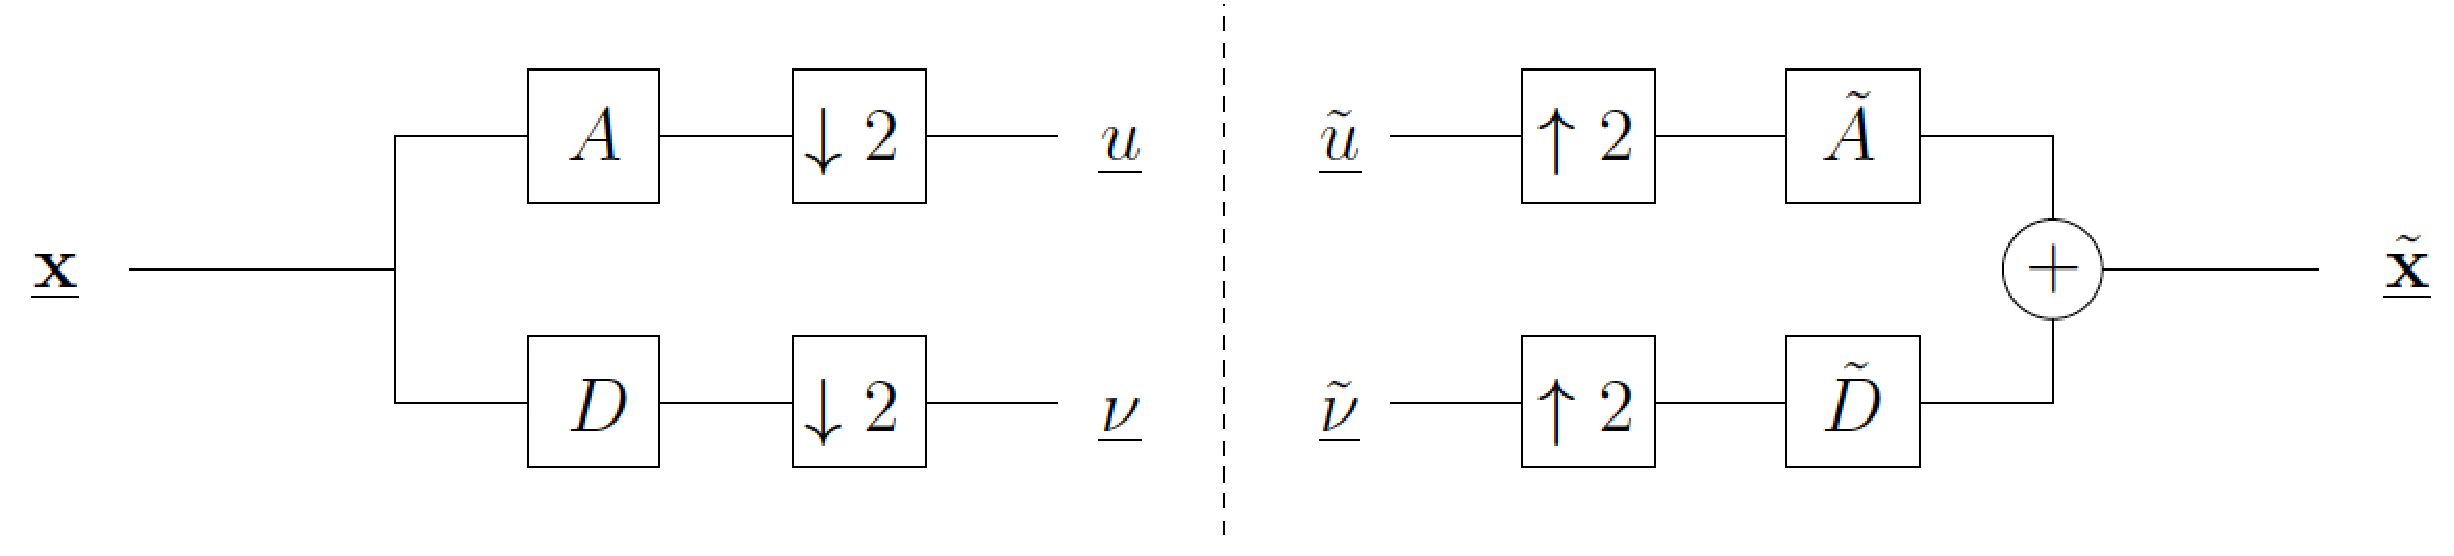
\includegraphics[width=0.5\textwidth]{content/FilterBank.pdf} 
\end{flushright}
 
\vspace{-0.5cm}

Filterbank (durch $-(-1)^k$ werden alle geraden Koeffizienten gelöscht ($=0$) ):
\[  
	\underbrace{\tilde{A}(z) A(z)}_{M(z)} + \underbrace{\tilde{D}(z)D(z)}_{-(-1)^k M(-z)} = M(z)-(-1)^kM(-z) = 2
	\qquad \qquad
	\tilde{A}(z)A(-z) + \tilde{D}(z)D(-z) = 0
\]

(Übung 9 (FS2013)-2a,b): Aus diesen Gleichungen folgt das Gleichungssystem:
\begin{align*}
  \text{Gleichung links, Koeffizient } z^0: \qquad & \tilde a_0 a_0 + \tilde a_1 a_{-1} + \tilde d_0 d_0 + \tilde d_1 d_{-1} &= 2 \\
  \text{Gleichung links, Koeffizient } z^1: \qquad & \tilde a_1 a_0 + \tilde d_1 d_0 &= 0 \\
  \text{Gleichung links, Koeffizient } z^{-1}: \qquad & \tilde a_0 a_{-1} + \tilde d_0 d_{-1} &= 0 \\
  \text{Gleichung rechts, Koeffizient } z^{0}: \qquad & \tilde a_0 a_0 - \tilde a_1 a_{-1} + \tilde d_0 d_0 - \tilde d_1 a_{-1} &= 0 \\
\end{align*}
und daraus die Koeffizienten:
\[
  \begin{pmatrix}
    \tilde a_0 & \tilde a_1\\
    \tilde d_0 & \tilde d_1
  \end{pmatrix}
  = \frac{1}{a_0 d_{-1} - a_{-1} d_0} \begin{pmatrix}
    d_{-1} & -d_0 \\
    -a_{-1} & a_0
  \end{pmatrix}
\]

Perfekte Rekonstruktion mit:
\[
\tilde{X}(z) = \frac12 \left( \big(A(z) X(z) + A(-z)X(-z)\big) \tilde{A}(z) + \big(D(z)X(z) + D(-z)X(-z)\big) \tilde{D}(z) \right)
\]
und im Falle von Haar: 
$A(z) = \frac{1+z}{\sqrt{2}} \quad 
D(z) = \frac{1-z}{\sqrt{2}} \quad 
\tilde{A}(z) = \frac{1+z^{-1}}{\sqrt{2}} \quad 
\tilde{D}(z) = \frac{1-z^{-1}}{\sqrt{2}}$
\\

\newpage

\subsubsection{Orthogonale Filterkoeffizienten \baeni{52, 75}}

\begin{tabularx}{\textwidth}{X | p{9cm}}
Die Filterkoeffizienten $h_k$ werden so in die Filterbank gerechnet:\newline
$A := H', \, \tilde A := H,\, D := G', \; \tilde D := G$\newline
mit den Koeffizienten: $h'_k = h_{-k}$, $g_k = (-1)^k h_{l-k}$
& Schema: \newline
  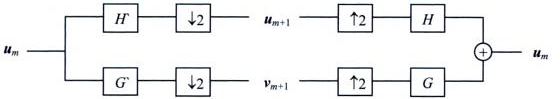
\includegraphics[width=9cm]{./content/MsaFilterbank.png}\\
\end{tabularx}\\
\\

Zusammenhang der Filter (shift: $(-z)^k$, inverse Reihenfolge durch $z^{-1}$, alternierendes Vorzeichen$(\pm)$ durch einsetzen von $-z$):
%TODO wo ist z^0 und wo z^n (Skript seite 27 + application db2 vergleichen???)
\[  
	\tilde{A}(z) = A(z^{-1})
	\qquad
	D(z) = \tilde{D}(z^{-1}) = (-z)^l\tilde{A}(-z) \qquad \tilde{D}(z) = (-z)^{-l}A(-z) \qquad l\text{: ungerade, frei wählbar}
\]
\[  
	A = [h_0,...,h_n] \qquad
	\tilde{A} = [h_n,...,h_0]
	\qquad \qquad
	D = [h_n,-h_{n-1}, h_{n-2},...,h_1,-h_0] \qquad
	\tilde{D} = [-h_0,h_1, -h_2,...,-h_{n-1},h_n]
\]

Mit einer orthogonalen Filterbank hat man Quadrature Mirror Filter Eigenschaften:\\
 $|\hat{h}(\xi)|^2 + |\hat{g}(\xi)|^2 = |\hat{\tilde{h}}(\xi)|^2 + |\hat{\tilde{g}}(\xi)|^2 = 2 \qquad \Leftrightarrow \qquad
 |\hat{a}(\xi)|^2 + |\hat{d}(\xi)|^2 = |\hat{\tilde{a}}(\xi)|^2 + |\hat{\tilde{d}}(\xi)|^2 = 2$

\subsubsection{Biorthogonale Filterkoeffizienten \baeni{78}}
Die Filterkoeffizienten $h_k, g_k$ werden so in die Filterbank gerechnet:\newline
$A := H', \, \tilde A := \tilde H,\, D := G', \; \tilde D := \tilde G$\\
\\

Zusammenhang der Filter (shift: $(-z)^k$ bzw. $-z^{-k}$, alternierendes Vorzeichen$(\pm)$ durch einsetzen von $-z$):
%TODO wo ist z^0 und wo z^n (Skript seite 27 + application db2 vergleichen???)
\[ 
	D(z) = (-z)^{l}\tilde{A}(-z) \qquad \qquad \tilde{D}(z) = (-z)^{-l}A(-z)  \qquad l\text{: ungerade, frei wählbar}
\]


	
	%Anhang
	\newpage
	\appendix
	\section{Lineare Algebra}

\subsection{Vektoren}

\subsubsection{Betrag von Vektoren}
\[ 
	|\vec{a}| = \sqrt{\vec{a} \cdot \vec{a}} = ||\vec{a}|| =\sqrt{a_1^2 + a_2^2 + \ldots + a_n^2}
\]

	
\subsubsection{Skalarprodukt}
\[ 
	\vec{a} \cdot \vec{b} = a_1 \cdot b_1 + a_2 \cdot b_2 + \ldots +a_n \cdot b_n = |\vec{a}| \cdot |\vec{b}| \cdot \cos(\varphi)
\]
			
Projektion $\vec{p}$ vom Vektor $\vec{a}$ auf den Einheitsvektor $\vec{e}$ (wobei $|\vec{e}|=1$): \hspace{1cm} $\vec{p}=(\vec{a} \cdot \vec{e}) \cdot \vec{e}$


\subsubsection{Vektorprodukt}
\[
	\vec{a} \times \vec{b} = 
	\begin{pmatrix}a_1\\a_2\\a_3 \end{pmatrix} \times 
	\begin{pmatrix}b_1\\b_2\\b_3 \end{pmatrix} = 
	\begin{pmatrix}
	a_2 b_3 - a_3 b_2 \\ \mathbf{a_3 b_1 -  a_1 b_3} \\ a_1 b_2 - a_2 b_1 
	\end{pmatrix} \quad \quad 
	|\vec{a} \times \vec{b}|=|\vec{a}| \cdot |\vec{b}| \cdot
	\sin(\varphi)
\]

Der Betrag von $|\vec{a} \times \vec{b}|$ entspricht der Fläche des
Parallelogramms das von $\vec{a}$ und $\vec{b}$ aufgespannt wird. Der Vektor  $\vec{a} \times \vec{b}$ steht senkrecht auf den Vektoren $\vec{a}$ und $\vec{b}$!

	
\subsection{Matrizen}

\subsubsection{Matrizenprodukt}
Matrizenprodukt (Skalarprodukt) einer Matrix A und einer Matrix B ergiebt eine
Matrix C, deren Elemente die Skalarprodukte der Zeilenvektoren von A mit den
Spaltenvektoren von B sind.

\[
	\begin{pmatrix}
	a_{11} & \ldots & a_{1n} \\
	\vdots & A & \vdots \\
	a_{n1} & \ldots & a_{nn}
	\end{pmatrix} \cdot \begin{pmatrix} 
	b_{11} & \ldots & b_{1n} \\
	\vdots & B & \vdots \\
	b_{n1} & \ldots & b_{nn}
	\end{pmatrix} = \begin{pmatrix}
	\sum\limits_{i=1}^n a_{1i}b_{i1} & \ldots & \sum\limits_{i=1}^n a_{1i}b_{in}
	\\ \vdots & C & \vdots \\
	\sum\limits_{i=1}^n a_{ni}b_{i1} & \ldots & \sum\limits_{i=1}^n a_{ni}b_{in}
	\end{pmatrix}
\]


\subsubsection{Rang}
Der Rang einer Matrix gibt an, wie viele Zeilen linear unabhängig sind.


\subsubsection{Spur}
Die Spur einer Matrix $A$ wird durch die Summe der Diagonalelemente berechnet.

\[
	\mathrm{Spur}(A)=\mathrm{tr}(A)=\sum\limits_{i=1}^n a_{ii}
\]

Rechenregeln:\\
- $\mathrm{Spur}(A)=\mathrm{Spur}(A^t)$\\
- $\mathrm{Spur}(AB)=\mathrm{Spur}(BA)$\\
- $\mathrm{Spur}(ABC)=\mathrm{Spur}(CBA)=\mathrm{Spur}(BCA)$\\

Anwendung: $\mathrm{Spur}(A)=1+2 \cos(\alpha)$

\subsubsection{Transponierte Matrix}
Transponierte Matrix $A^t$ heisst alle Spalten und Zeilen
der Matrix $A$ vertauschen.

\[
	A=  
	\begin{pmatrix} 
		a_{11} & a_{12} & \cdots & a_{1n} \\
		a_{21} & a_{22} & \cdots & a_{2n} \\
		\vdots & \vdots & \ddots & \vdots \\
		a_{m1} & a_{m2} & \cdots & a_{mn} \\
	\end{pmatrix}
	\qquad \qquad 
	A^{\mathrm{T}} = 
	\begin{pmatrix} 
		a_{11} & a_{21} & \cdots & a_{m1} \\
		a_{12} & a_{22} & \cdots & a_{2n} \\
		\vdots & \vdots & \ddots & \vdots \\
		a_{1n} & a_{2n} & \cdots & a_{mn} \\
	\end{pmatrix}
\]

Rechenregeln:\\
- $(A+B)^t=A^t+B^t$\\
- $(A \cdot B)^t=B^t \cdot A^t$


\subsubsection{Orthogonale Matrix}
Eigenschaften:\\
- Quadratisch\\
- Zeilenvektoren sind orthonormal, Spaltenvektoren sind orthonormal\\
- Multiplikation von 2 orthogonalen Matrizen gibt eine orthogonale
Matrix\\
- $A^t=A^{-1}$ und $A^t \cdot A = I$(Einheitsmatrix)\\
- Determinante hat immer Betrag $1$\\
- $\det(O)=+1$: die orthogonale Matrix $O$ enthält alle Drehungen\\
- $\det(O)=-1$: die orthogonale Matrix $O$ enthält alle Drehspiegelungen 


\subsubsection{Determinante (Quadratische Matrizen)}
\textbf{Berechnung:} \\
Die Determinante ist das Produkt der Pivoelemente $p$ (mit
Gauss ermittelbar).  $\det \begin{pmatrix}p_1 & \ldots & \ast \\
\vdots & p_i & \vdots \\ \ast & \ldots & p_n \end{pmatrix} =
\sum\limits_{i=1}^{n}p_i$\\

2D Matrix (Fisch): \hspace{1cm} $\det \begin{pmatrix}a & b \\ c
& d \end{pmatrix} = a d - b c$\\

\textbf{Rechenregeln:}\\
- $\det(A \cdot B) = \det(A) \cdot \det(B)$\\
- $\det(A^{-1})=\det(A)^{-1}=\frac{1}{\det(A)}$\\
- $\det(A^t)=\det(A)$ wenn $A$ Quadratische \\

\textbf{Merksätze:}\\
- Matrix $A$ linear abhängig $\Rightarrow \det(A)=0$\\
- Vertauschen von 2 Zeilen $\Rightarrow (-1)\cdot \det(A)$\\
- Determinante einer 2D Matrix entspricht der Fläche des aufgespannten
Parallelogramm\\
- Determinante einer 3D Matrix entspricht dem Volumen des aufgespannten
Parallelepipeds\\
- Determinante einer orthagonalen Matrix hat immer Betrag $1$

\subsubsection{Matrixinversion}
	$A^{-1} = \begin{pmatrix}
	a & b \\ c & d \\
	\end{pmatrix}^{-1} =
	\frac{1}{\det(A)} \begin{pmatrix}
	d & -b \\ -c & a \\
	\end{pmatrix}  =
	\frac{1}{ad-bc} \begin{pmatrix}
	d & -b \\ -c & a \\
	\end{pmatrix}\quad$\\
	$A^{-1} = \begin{pmatrix}
	a & b & c\\ d & e & f \\ g & h & i \\
	\end{pmatrix}^{-1} =
	\frac{1}{\det(A)} \begin{pmatrix}
	ei - fh & ch - bi & bf - ce \\
	fg - di & ai - cg & cd - af \\
	dh - eg & bg - ah & ae - bd
	\end{pmatrix}$\\

\subsubsection{Cramersche Regel}
Ausgangslage: $\qquad A \cdot x = b \qquad \det(A)\neq 0$\\
Lösung $x_i$:
\[
	x_i=\frac{\det(A_i)}{\det(A)} \qquad \qquad A_i:\text{ $i$-te Spalte von $A$  durch rechte Seite  $b$ ersetzen!}
\]


\subsection{Eigenvektoren und Eigenwerte}
Ein Eigenvektor $v$ einer Abbildung $A$ (Matrix) ist ein vom Nullvektor
verschiedener Vektor, dessen Richtung durch die Abbildung nicht verändert wird. Der Vektor wird nur
gestreckt oder gestaucht. Dieser Faktor wird Eigenwert $\lambda$ genannt.
\[
	A v = \lambda v \quad \Leftrightarrow \quad (A-\lambda I)v=0
\]

\textbf{Charakteristisches Polynom:}\\
\[
	\chi_A(\lambda)=\det(A-\lambda I)
\]

\textbf{Eigenwerte:}\\
Die Nullstelle (da $A-\lambda I$ Singulär) des charakteristischen Polynom sind
die Eigenwerte. 
\[
	\chi_A(\lambda)=\det(A-\lambda I)=0
\]

\textbf{Eigenvektoren:}\\
Um die Eigenvektoren zu erhalten muss das folgende Gleichungssystem für jeden
Eigenwert gelöst werden.
\[ 
	(A-\lambda I)v=0 \qquad \qquad (v \text{ auf länge 1 normieren})
\]

\subsection{Spezielle Matrizen}
Einheitsmatrix: 
$I= \begin{pmatrix} 
1 & 0 & 0 \\
0 & 1 & 0 \\
0 & 0 & 1
\end{pmatrix}$

\vspace{0.5cm}

Drehmatrizen:
\\
$\quad$
X-Achse
$\begin{pmatrix} 
	1 & 0 & 0 \\
	0 & \cos(\alpha) & -\sin(\alpha) \\
	0 & \sin(\alpha) & \cos(\alpha)
\end{pmatrix}$
$\quad$
Y-Achse
$\begin{pmatrix} 
	\cos(\alpha) & 0 & \sin(\alpha) \\
	0 & 1 & 0 \\
	-\sin(\alpha) & 0 & \cos(\alpha)
\end{pmatrix}$
$\quad$
Z-Achse
$\begin{pmatrix} 
	\cos(\alpha) & -\sin(\alpha) & 0 \\
	\sin(\alpha) & \cos(\alpha) & 0 \\
	0 & 0 & 1
\end{pmatrix}$

	\newpage
	\input{content/appendix/FourierReihe.tex}
	\section{Fourier Transformation}
\[
\boxed{f(t) =  \frac{1}{2\pi}\int\limits_{-\infty}^{\infty}
F(\omega)e^{j\omega t}d\omega}=\frac{1}{2
\pi}\int\limits_{-\infty}^{\infty}(R(\omega) \cos(\omega t) + X(\omega)
\sin(\omega t))d\omega + \frac{j}{2 \pi}\int \limits_{-
\infty}^{\infty}(R(\omega) \sin(\omega t)- X(\omega) \cos(\omega t))d\omega
\]

\[	
\boxed{F(\omega) = \int\limits_{-\infty}^{\infty} f(t)e^{-j\omega t}dt}
= R(\omega) - j X(\omega) \quad R(\omega) = \int\limits_{-\infty}^{\infty}
f(t)\cos(\omega t)dt \quad \mbox{ und } \quad X(\omega)=
\int\limits_{-\infty}^{\infty}f(t)\sin(\omega t)dt 
\]

\subsection{Spektren}
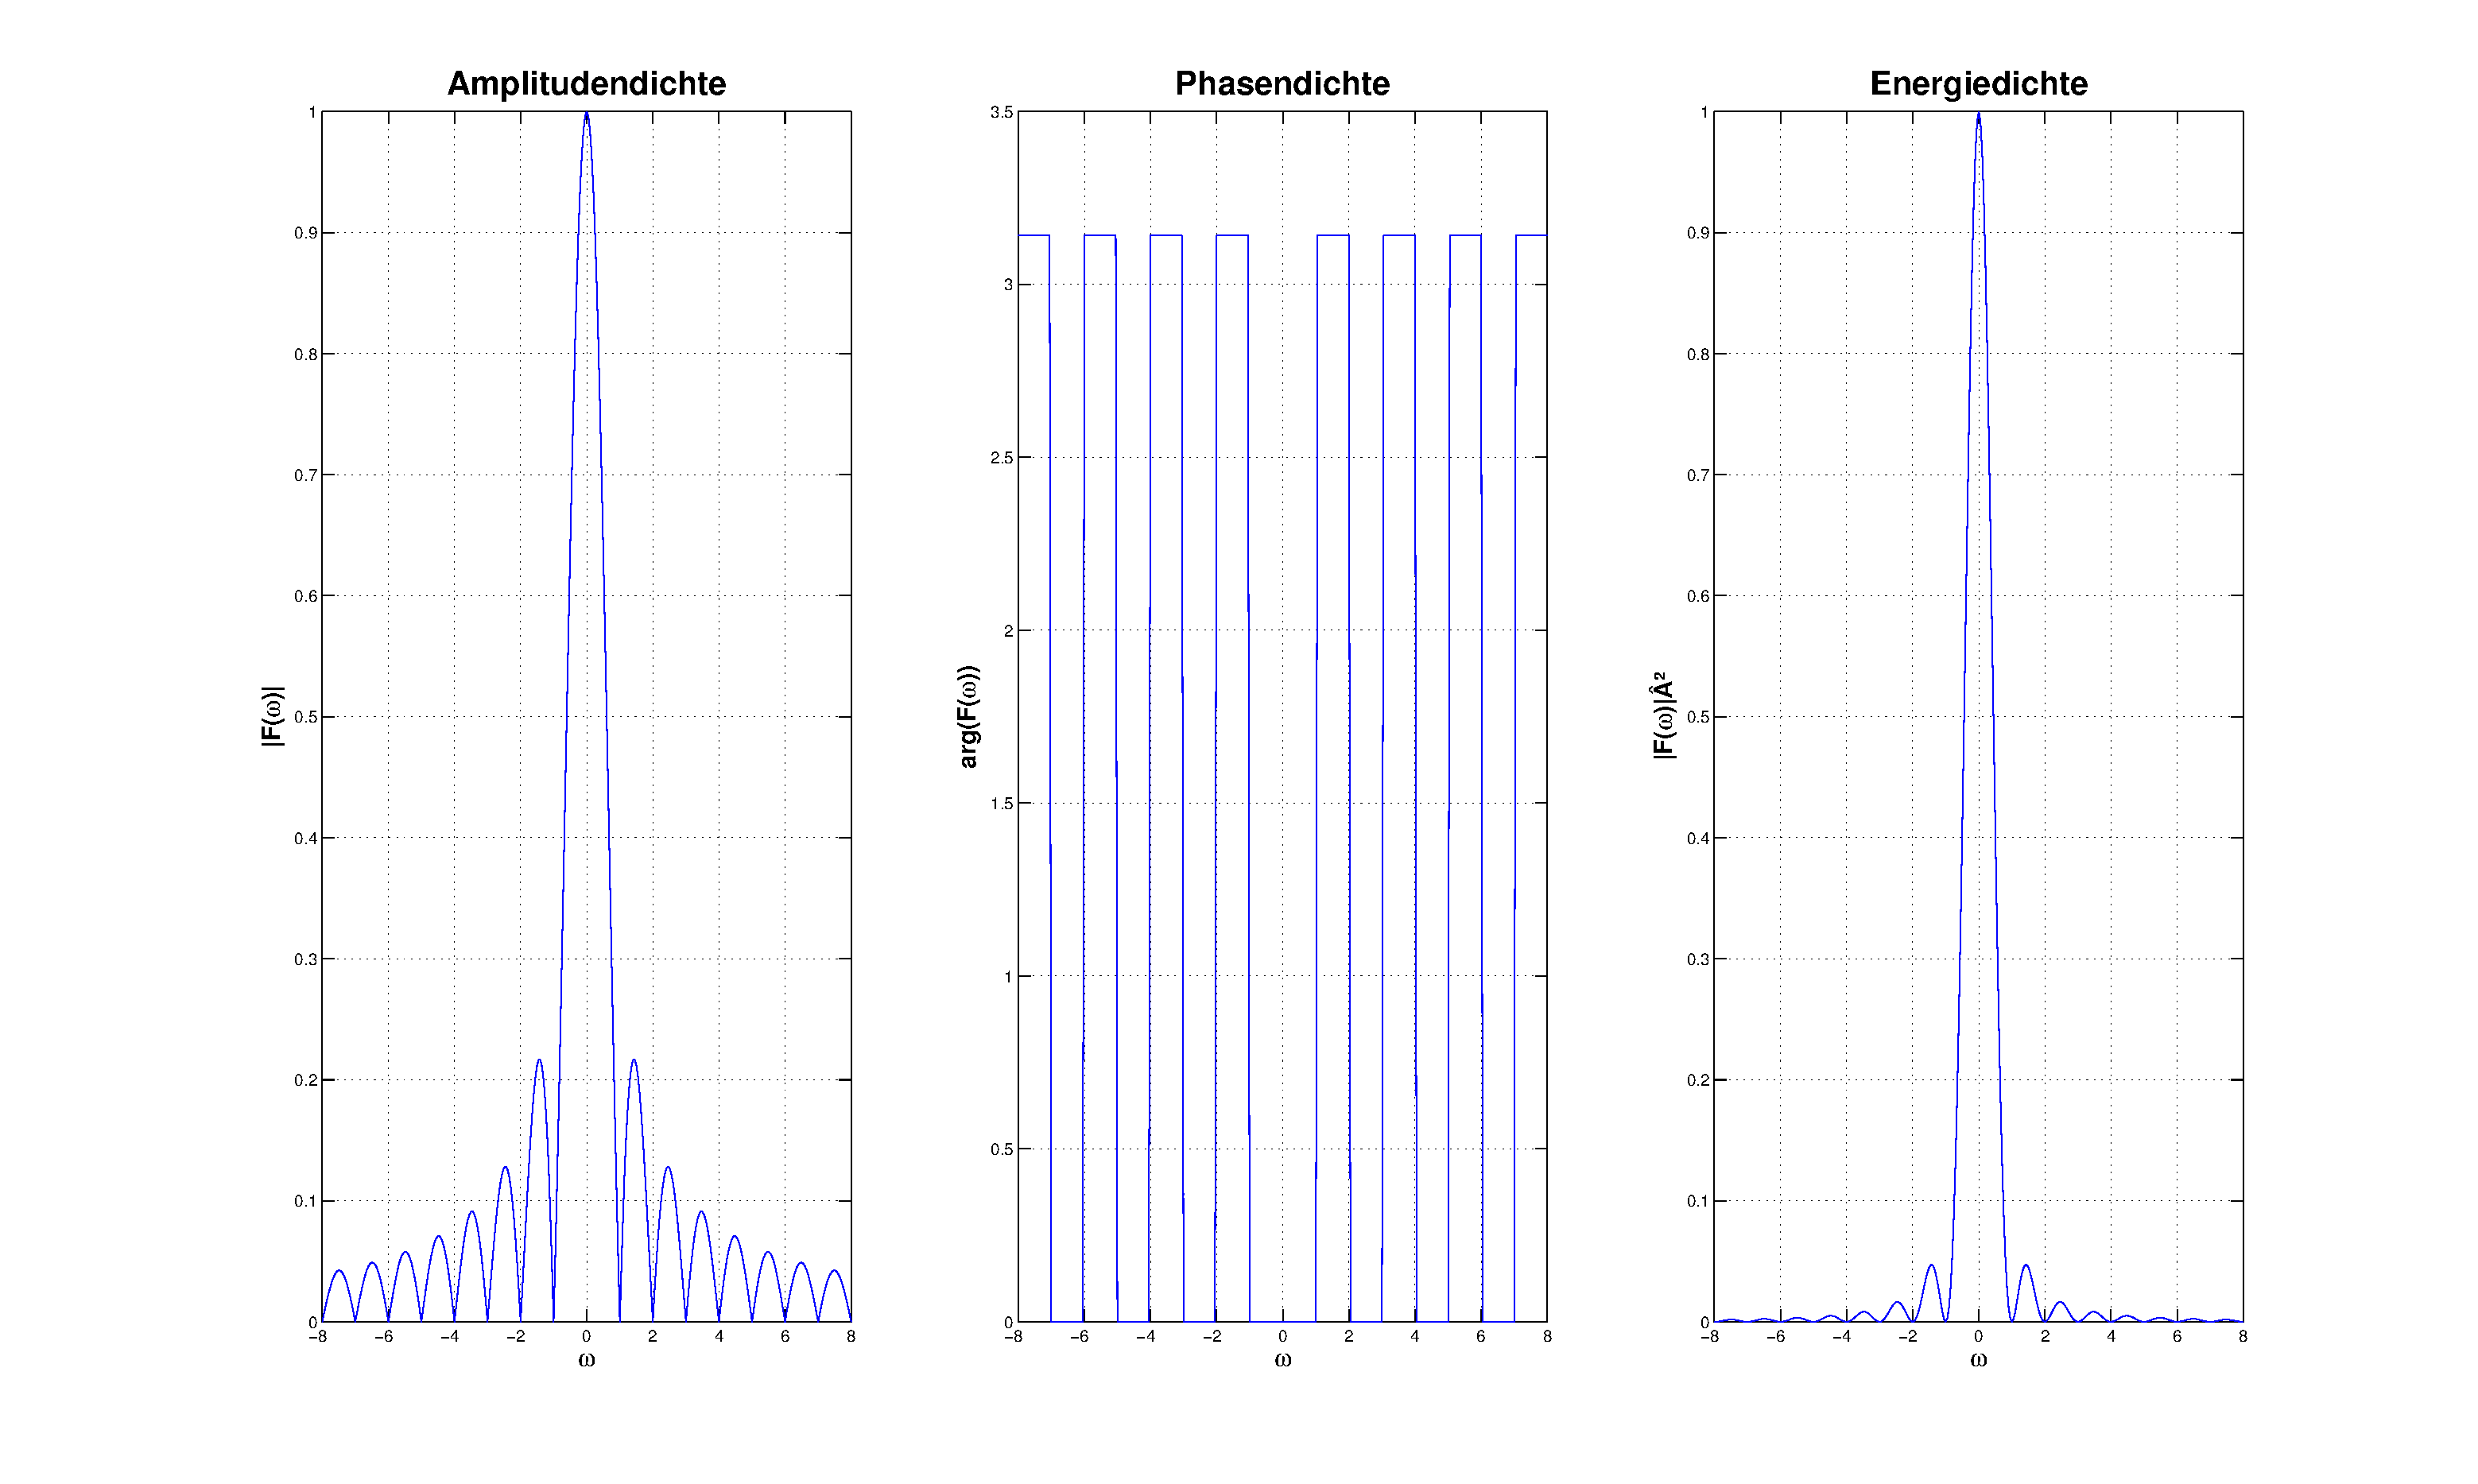
\includegraphics[width=0.8\textwidth,trim=1cm 1cm 1cm 1cm]{content/appendix/Spektern.pdf}

\newpage	
\subsection{Eigenschaften}
Fourierintegral existiert wenn  $\int\limits_{-\infty}^{\infty}|f(t)| dt < \infty$\\

\renewcommand{\arraystretch}{2}

\begin{tabular}{|p{8cm}|l c l|}
  \hline
 	Linearität & 
 	$\alpha\cdot f(t) + \beta\cdot g(t)$ & $\FT$ & $\alpha\cdot F(\omega) + \beta\cdot G(\omega)$\\
 	\hline
  Zeitumkehrung (Spiegelung an der Y-Achse)&
  $f(-t)$ & $\FT$ & $F(-\omega) = F^*(\omega)$ \\
	\hline        	
	Ähnlichkeit &
	$f(\alpha t)$ & $\FT$ & $\frac{1}{|\alpha|}F \left (\frac{\omega}{\alpha} \right) \quad\alpha \in\mathbb{R}\setminus \{0\}$\\
	\hline
	Verschiebung im	Zeitbereich &
	$f(t\pm t_0)$ & $\FT$ & $F(\omega)e^{\pm j\omega t_0}$\\
	\hline
  Verschiebung im Frequenzbereich &
	$f(t)e^{\pm j\omega_0 t}$ & $\FT$ & $F(\omega\mp\omega_0)$\\
	\hline
	Ableitung im Zeitbereich &
	$\frac{\partial^n f(t)}{\partial t^n}$ & $\FT$ & $(j\omega)^n F(\omega)$\\
	\hline
	Integration im Zeitbereich &
	$\int\limits_{-\infty}^{t}f(\tau)d\tau $ & $\FT$ & 
	$\frac{F(\omega)}{j\omega}+\pi F(0)\delta(\omega)$\\
	\hline				
	Ableitung im Frequenzbereich &
	$t^n f(t)$ & $\FT$ & $j^n \frac{\partial F(\omega)}{\partial \omega^n}$\\
	\hline		
	Faltung im Zeitbereich &
	$f(t) \ast g(t)$ & $\FT$ & $F(\omega) \cdot G(\omega)$\\
	\hline
	Faltung im Frequenzbereich &
	$f(t) \cdot g(t)$ & $\FT$ & $\frac{1}{2\pi}F(\omega) \ast G(j\omega)$\\
	\hline
	Vertauschungssatz (Dualität) &
	$f(t)$ & $\FT$ & $F(\omega)\nonumber$ \\
	& $F(t)$ & $\FT$ & $2\pi \cdot f(-\omega)$\\
	\hline
	Modulation &
	$\cos(\alpha t) \cdot f(t)$ & $\FT$ & $\frac{1}{2}\cdot \left[F(\omega-\alpha) + F(\omega+\alpha)\right ]$\\
	& $\sin(\alpha t) \cdot f(t)$ & $\FT$ & $\frac{1}{2j}\cdot \left[	F(\omega-\alpha) - F(\omega+\alpha)\right ]$\\
	\hline
 	Parseval's Theorem &
  $\int\limits_{-\infty}^{\infty}f(t)g^{\ast}(t)dt $ & $=$ & $ \frac{1}{2\pi}	\int\limits_{-\infty}^{\infty}F(\omega)G^{\ast}(\omega)d\omega$\\
	\hline
	Bessel's Theorem (Satz von Parseval) &
	$\int\limits_{-\infty}^{\infty}|f(t)|^2 dt $ & $=$ & $ \frac{1}{2\pi}\int\limits_{-\infty}^{\infty}|F(\omega)|^2 d\omega$\\
	\hline 			
  Anfangswerte &
  $f(0)=\frac{1}{2\pi}\int\limits_{-\infty}^{\infty}F(\omega)d\omega$ 
  && $ F(0)=\int\limits_{-\infty}^{\infty}f(t)dt$\\
	\hline
	$\infty$ lange Folge von $\delta$-Impulsen &
	$\sum\limits_{n=-\infty}^{\infty} \delta(t-n\cdot t_0)$ & $\FT$ & 
	$\sum\limits_{n=-\infty}^{\infty} \frac{2\pi}{t_0}\delta(\omega-n\cdot \frac{2\pi}{t_0})$\\
	\hline
\end{tabular}
\renewcommand{\arraystretch}{1}


\subsection{Wichtige Fourier Transformationspaare}
\begin{landscape}
\begin{center}
\renewcommand{\arraystretch}{2.5}
\begin{tabular}{|rll|rll|}
\hline
    $x(t)$ & $\FT$ & $X(\omega)$ &
    $\e^{-a \cdot t} \cdot \text{u}(t) ~~~~ a > 0$ & $\FT$ & $\frac{1}{j\omega + a}$
  \\ \hline
    $\delta(t)$ & $\FT$ & $1$ &
    $t \cdot \e^{-a \cdot t} \cdot \text{u}(t) ~~~~ a > 0$ & $\FT$ & $\frac{1}{(j\omega + a)^2}$
  \\ \hline
    $\delta(t-t_0)$ & $\FT$ & $e^{-j\omega t_0}$
    & $t^n$ &$\FT$& $2 \pi j^n \delta^{(n)}(\omega) ~~~~ (n=1,2,...)$ 
  \\ \hline
    $1$ & $\FT$ & $2 \pi \cdot \delta(\omega)$ &
    $\e^{-a \cdot |t|} ~~~~ a > 0$ & $\FT$ & $\frac{2a}{\omega^2 + a^2}$
  \\ \hline
    $\text{u}(t)=\sigma(t)$ & $\FT$ & $\pi \cdot \delta(\omega) + \frac{1}{j\omega}$ &
    $\e^{\frac{-t^2}{(2\sigma)^2}}$ & $\FT$ & $\sigma \sqrt{2\pi} \cdot
    \e^{\frac{-\sigma^2 \cdot \omega^2}{2}}$
  \\ \hline
    $\text{sgn}(t)$ & $\FT$ & $\frac{2}{j\omega}$ &
    $\sinc(a t)=\frac{\sin(a t)}{a t}$ & $\FT$ & $\frac{\pi}{a} \cdot \text{p}_a(\omega)=\begin{cases} 1 \cdot \frac{\pi}{a} &
    |\omega| < a \\ 0 & |\omega| > a \end{cases} $
  \\ \hline
    $\frac{1}{\pi \cdot t}$ & $\FT$ & $-j \cdot \text{sgn}(\omega)$ &
    $\text{p}_a(t)=\begin{cases} 1 & |t| < a \\ 0 & |t| > a \end{cases} $ & $\FT$ & $2
    \cdot a \cdot \frac{\sin(\omega \cdot a)}{\omega a} = 2a \sinc{a \omega}$
  \\ \hline
    $\e^{j \omega_0 t}$ & $\FT$ & $2 \pi \cdot \delta(\omega - \omega_0)$ 
     & $x(t) = \begin{cases} 1 - \frac{|t|}{a} & |t| < a \\ 0 & |t| > a \end{cases}$
     & $\FT$ & $a \cdot \left ( \frac{\sin(\frac{\omega \cdot a}{2})}{\frac{\omega \cdot a}{2}} \right )^2$
  \\ \hline
    $\cos(\omega_0 t)$ & $\FT$ & $\pi \cdot \left ( \delta(\omega - \omega_0) + \delta(\omega + \omega_0) \right )$ 
    &$\delta^{(n)}(t)$ &$\FT$ & $(j\omega)^n$
  \\ \hline
    $\sin(\omega_0 t)$ & $\FT$ & $-j\cdot \pi \cdot \left ( \delta(\omega - \omega_0) - \delta(\omega + \omega_0) \right )$ 
    & $\delta^{(n)}(t-a)$&$\FT$ & $(j\omega)^n \e^{-j\omega a} ~~~~ (n=1,2,...)$
  \\ \hline
    $\hat{x}(t) = \frac{1}{\pi}\int\limits_{-\infty}^{\infty} \frac{x(\tau)}{t -
    \tau} d\tau$ & $\FT$ & $-j\cdot \text{sgn}(\omega) \cdot X(\omega)$ &
    $\sum \limits_{n=-\infty}^{\infty} \delta(t-n \cdot T) $ & $\FT$ & $\omega_0
    \sum \limits_{n=-\infty}^{\infty} \delta(\omega - n\cdot \omega_0) $
  \\ \hline
\end{tabular}
\renewcommand{\arraystretch}{1}
\end{center}
\end{landscape}
  
  
\subsection{Fourierreihe durch periodisches Fortsetzen der Fouriertransformation}
\[
s(t) = \sum\limits_{n=-\infty}^{\infty} c_n \e^{j\omega_0 n t} \FT S(\omega) = 2\pi \sum\limits_{n=-\infty}^{\infty}c_n \delta(\omega - n\omega_0)
= \omega_0 S_0(\omega) \sum\limits_{n=-\infty}^{\infty} \delta(\omega-n\omega_0)
\] 

\[
c_n = \frac{1}{T}S_0(n\omega_0) \text{ wobei } \omega_0 = \frac{2\pi}{T} \text{ und } S_0(\omega) \IFT s_0(t)
\]

\begin{tabular}{L{9cm}C{9cm}}
$s_0(t)$ stellt eine Periode des Signals $s(t)$ mit Fourierreihe
& \multirow{2}{12cm}{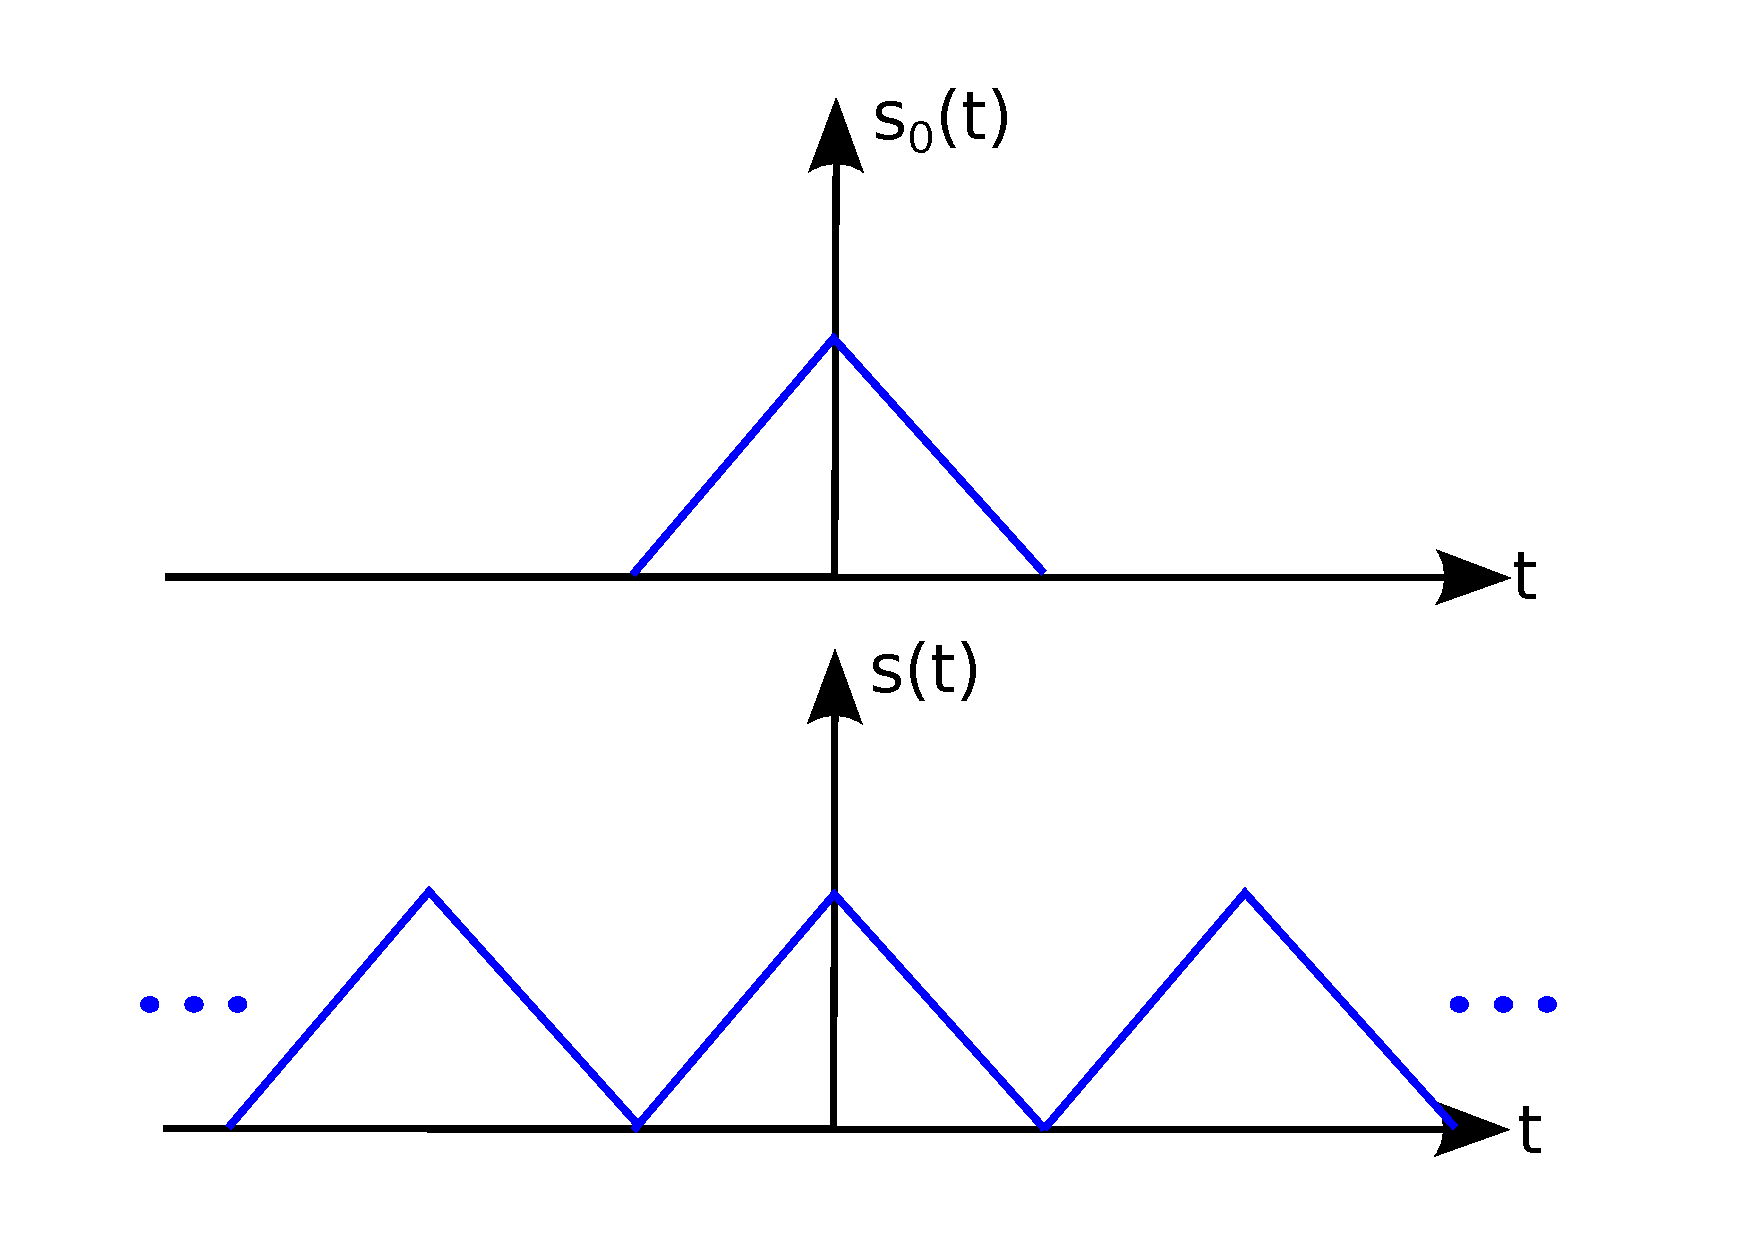
\includegraphics[width=0.25\textwidth]{content/appendix/FTperiodisch.pdf}} \\
$s(t) = \sum c_n \e^{jn\omega_0}$ dar. & \\
\end{tabular}	

	\section{Faltung}
Faltung:
\begin{equation}
  \nonumber
  y(t) = f(t) \ast g(t) = \int\limits_{-\infty}^{\infty}f(u) \cdot g(t-u) du
\end{equation}

Periodisch:
\begin{equation}
  \nonumber
  y(t) = f(t) \ast g(t) = \frac{1}{T}\int\limits_{a}^{a + T}f(u) \cdot g(t-u) du
\end{equation}

Diskret:
\begin{equation}
  \nonumber
  y(i)=f(i) \ast g(i)=\sum\limits_{k=-\infty}^{\infty}f(k)\cdot g(i-k)
\end{equation}

\begin{tabular}{p{9cm}p{9cm}}
  Interpretation: & Geltende Rechengesetze:\\
  \begin{enumerate}
    \item $g(t)$ an der Y-Achse Spiegeln
	  \item Verschiebung um $t$ nach rechts
	  \item Durch Multiplikation der beiden Signale entstehende Fläche berechnen
  \end{enumerate}
&
  \begin{itemize}
    \item Kommutativ (Vertauschen) $g \ast f = f \ast g $
	  \item Distributiv (Ausklammern, Ausmultiplizieren) $g \ast(f \ast h) = g \ast f \ast h$
	  \item Assoziativ (Reihenfolge von Klammern) $g \ast(f \ast h) = (g \ast f) \ast h$
	  \item Faltung mit Dirac $\delta(t-t_0) \ast f(t) = f(t-t_0)$
  \end{itemize}
\end{tabular}
	
	
	

	
\end{document}